

\begin{figure}[!h]
    \centering
    \resizebox{!}{0.95\textwidth}{
        \begin{tikzpicture}[mindmap,
        level 1 concept/.append style={level distance=130,sibling angle=90},
        ]
        \path[mindmap,concept color=black,text=white]
        node[concept] {Function}
        [clockwise from=-90]
        child[concept color=blue,sibling angle=60,text=black] {
            node[concept] (graphs) {Equations and Graphs}
            [clockwise from=-35]
            child { node[concept] (intercepts) {Intercepts} }
            child { node[concept] (shift) {Shifts} }
            child { node[concept] (scale) {Scaling} }
        }
        child[concept color=red,text=black]{
          node[concept] (special) {Polynomials}
          [clockwise from=240]
          child[concept color=red] {
            node[concept] (lines) {Linear}
            [clockwise from=270]
            child { node[concept] (linearRate) {Rates} }
            child { node[concept] (lineForms) {Different Forms} }
          }
          child[concept color=red] {
            node[concept] (quadratics) {Quadratics}
            [clockwise from=90]
            child { node[concept] (quadVertex) {Vertex} }
            child { node[concept] (quadMinMax) {Max/Min} }
          }
        }
        child[concept color=black,sibling angle=75] {
            node[concept] (rangeDomain) {Range / Domain}
        }
        child[concept color=black,sibling angle=-50] {
            node[concept] (operations) {Operations}
            [clockwise from=90,sibling angle=90]
            child[concept color=black] {
                node[concept] (composition) {Compositions}
            }
        };

        \begin{scope}[concept color=green!50!black]
        \node[extra concept,color=green!50!black,circle,font=\scriptsize,text=black,level distance=10]
             (coord) at (4,0) {Coordinate System}
             [clockwise from=0]
             child[concept color=green!50!black,level distance=70] {
                 node[concept] (distanceFormula) {Distance Formula}
%                 [clockwise from=-90]
%                 child {
%                    node[concept,color=green!50!black,text=black] (circles) {Circles and Semi-Circles}
%                    [clockwise from=-90,sibling angle=90]
%                    child { node[concept] {Radius} }
%                    child { node[concept] {Center} }
%              }
        };
      \end{scope}


        \begin{pgfonlayer}{background}
        \draw [left color=black, right color=black, draw=white,
               decorate,decoration=circle connection bar]
               (rangeDomain) -- (composition);
        \draw [left color=black, right color=green, draw=white,
               decorate,decoration=circle connection bar]
               (rangeDomain) -- (coord);
        \draw [left color=black, right color=blue, draw=white,
               decorate,decoration=circle connection bar]
               (rangeDomain) -- (graphs);
        \draw [left color=blue, right color=blue, draw=white,
               decorate,decoration=circle connection bar]
               (shift) -- (scale);
        \draw [left color=red, right color=blue, draw=white,
               decorate,decoration=circle connection bar]
               (special) -- (graphs);
        \draw [left color=blue, right color=green, draw=white,
               decorate,decoration=circle connection bar]
               (graphs) -- (coord);
       \draw [left color=blue, right color=green, draw=white,
              decorate,decoration=circle connection bar]
              (intercepts) -- (coord);
        \end{pgfonlayer}


        \end{tikzpicture}
      }
      \caption{Topics for the first section of the course.}
\end{figure}


%=========================================================================
% Start of
%=========================================================================
\preClass{Coordinate Systems}

\begin{problem}
\item Make a sketch of a number line with zero at the center.  Mark
  the locations of -2, -2.5, 1.1, and 2.3 on your number line.
  The relative distances between the points should be consistent.
  \sideNote{Label the number line by putting an ``$x$'' to the right
    and an arrow indicating the positive direction.}

  \vfill

\item Make a sketch of a number line with zero at the center.  Mark
  the locations of -2 and 2.15 on your number line. What is the
  distance between the two points?
  (The relative distances between the points should be consistent.)

  \vfill

\item Make a sketch of a number line with zero at the center.  Mark
  the locations of -1.54 and 2.07 on your number line. What is the
  distance between the two points?
  (The relative distances between the points should be consistent.)

  \vfill

\end{problem}


\actTitle{Coordinate Systems}
\begin{problem}
\item A set of points is given below as a table. Each point is given
  on a line. The left side of the table has the $x$-coordinate of each
  point, and the right side has the $y$ coordinate. Plot each point on
  the axes given below. Next to each point indicate which quadrant the
  point is located.

  \begin{tabular}{l|ll}
    $x$ & $y$ & Quadrant \\ \hline
     2.0 &  1.5 & \\ [10pt]
     2.2 & -4.5 & \\ [10pt]
    -3.4 &  2.8 & \\ [10pt]
    -2.8 & -1.3 & \\ [10pt]
    -4.5 &  2.5 & \\ [10pt]
  \end{tabular}

  \begin{tikzpicture}[y=1cm, x=1cm,font=\sffamily]
    % bounds
    \def\lowX{-5.5}
    \pgfmathtruncatemacro\startX{round(0.5+\lowX)}
    \pgfmathsetmacro\nextXValue{int(\startX+1)}
    \def\highX{5.5}
    \def\lowY{-5.5}
    \def\highY{5.5}
    \pgfmathsetmacro\nextYValue{int(\lowY+1)}
    % ticks
    \draw[step = 1, gray, very thin,dashed,opacity=0.85] (\lowX, \lowY) grid ( \highX,\highY);
 	% axis
	\draw[thick,->] (\lowX,0) -- coordinate (x axis mid) (\highX,0) node[anchor = north west] {$x$};
    \draw[thick,->] (0,\lowY) -- coordinate (y axis mid) (0,\highY) node[anchor = south east] {$y$};
    \foreach \y in {-5,-4,...,-1,1,2,...,\highY} {
      \draw (1pt, \y) -- (-1pt, \y) node[yshift=-6,xshift=-1,anchor=east] {$\y$};
    }
    \foreach \x in {-5,-4,...,-1,1,2,...,\highX} {
      \draw (\x,1pt) -- (\x,-1pt) node[yshift=-5,xshift=-1,anchor=east] {$\x$};
    }
  \end{tikzpicture}

  \vfill

  \clearpage

\item Mark the points $P_1(-2.1,-4.4)$ and $P_2(4.5,1.2)$ on the coordinate plane
  below. Determine the distance between the two points.  Include a
  sketch of a right triangle whose hypotenuse represents the distance
  between the two points.

  \begin{tikzpicture}[y=1cm, x=1cm,font=\sffamily]
    % bounds
    \def\lowX{-5.5}
    \pgfmathtruncatemacro\startX{round(0.5+\lowX)}
    \pgfmathsetmacro\nextXValue{int(\startX+1)}
    \def\highX{5.5}
    \def\lowY{-5.5}
    \def\highY{5.5}
    \pgfmathsetmacro\nextYValue{int(\lowY+1)}
    % ticks
    \draw[step = 1, gray, very thin,dashed,opacity=0.85] (\lowX, \lowY) grid ( \highX,\highY);
 	% axis
	\draw[thick,->] (\lowX,0) -- coordinate (x axis mid) (\highX,0) node[anchor = north west] {$x$};
    \draw[thick,->] (0,\lowY) -- coordinate (y axis mid) (0,\highY) node[anchor = south east] {$y$};
    \foreach \y in {-5,-4,...,-1,1,2,...,\highY} {
      \draw (1pt, \y) -- (-1pt, \y) node[yshift=-6,xshift=-1,anchor=east] {$\y$};
    }
    \foreach \x in {-5,-4,...,-1,1,2,...,\highX} {
      \draw (\x,1pt) -- (\x,-1pt) node[yshift=-5,xshift=-1,anchor=east] {$\x$};
    }
  \end{tikzpicture}

  \vfill

  \clearpage

\item Mark the point $P_3(1.3,-2.4)$ on the coordinate plane below. Determine the
  points on the $x$-axis that are a distance of 3 units from $P_3$.

  \begin{tikzpicture}[y=1cm, x=1cm,font=\sffamily]
    % bounds
    \def\lowX{-5.5}
    \pgfmathtruncatemacro\startX{round(0.5+\lowX)}
    \pgfmathsetmacro\nextXValue{int(\startX+1)}
    \def\highX{5.5}
    \def\lowY{-5.5}
    \def\highY{5.5}
    \pgfmathsetmacro\nextYValue{int(\lowY+1)}
    % ticks
    \draw[step = 1, gray, very thin,dashed,opacity=0.85] (\lowX, \lowY) grid ( \highX,\highY);
 	% axis
	\draw[thick,->] (\lowX,0) -- coordinate (x axis mid) (\highX,0) node[anchor = north west] {$x$};
    \draw[thick,->] (0,\lowY) -- coordinate (y axis mid) (0,\highY) node[anchor = south east] {$y$};
    \foreach \y in {-5,-4,...,-1,1,2,...,\highY} {
      \draw (1pt, \y) -- (-1pt, \y) node[yshift=-6,xshift=-1,anchor=east] {$\y$};
    }
    \foreach \x in {-5,-4,...,-1,1,2,...,\highX} {
      \draw (\x,1pt) -- (\x,-1pt) node[yshift=-5,xshift=-1,anchor=east] {$\x$};
    }
  \end{tikzpicture}

  \vfill

  \begin{enumerate}
  \item Place points on the graphs near to where you think the points
    \textbf{may} be located.
  \item Label one of the points, $(x,y)$. 
  \item Write out the general distance formula.
  \item What do you know about the point? Can you simplify the formula?
  \item Solve for the unknown variable.
  \end{enumerate}

  \vfill


\clearpage

\item Mark the point $P_4(1,-2)$ on the coordinate plane below. Mark \textbf{all}
  of the points that are a distance of 2 units from $P_4$.

  \begin{tikzpicture}[y=1cm, x=1cm,font=\sffamily]
      % bounds
      \def\lowX{-5.5}
      \pgfmathtruncatemacro\startX{round(0.5+\lowX)}
      \pgfmathsetmacro\nextXValue{int(\startX+1)}
      \def\highX{5.5}
      \def\lowY{-5.5}
      \def\highY{5.5}
      \pgfmathsetmacro\nextYValue{int(\lowY+1)}
      % ticks
      \draw[step = 1, gray, very thin,dashed,opacity=0.85] (\lowX, \lowY) grid ( \highX,\highY);
   	% axis
  	\draw[thick,->] (\lowX,0) -- coordinate (x axis mid) (\highX,0) node[anchor = north west] {$x$};
      \draw[thick,->] (0,\lowY) -- coordinate (y axis mid) (0,\highY) node[anchor = south east] {$y$};
      \foreach \y in {-5,-4,...,-1,1,2,...,\highY} {
        \draw (1pt, \y) -- (-1pt, \y) node[yshift=-6,xshift=-1,anchor=east] {$\y$};
      }
      \foreach \x in {-5,-4,...,-1,1,2,...,\highX} {
        \draw (\x,1pt) -- (\x,-1pt) node[yshift=-5,xshift=-1,anchor=east] {$\x$};
      }
    \end{tikzpicture}

  \vfill

  What kind of figure did you draw?

  \vfill

\clearpage

\item Suppose a point, $P(x,y)$ is a distance of 2 units from the
  point $P_4(1,-2)$.
  \begin{subproblem}
  \item Use the distance formula to express the distance relationship
    between $P$ and $P_4$.
    \vfill
  \item Square both sides of the previous equation.
    \vfill
  \end{subproblem}

\item Suppose a point, $P(x,y)$ is a distance of $R$ units from the
  point $P_4(1,-2)$.
  \begin{subproblem}
  \item Use the distance formula to express the distance relationship
    between $P$ and $P_4$.
    \vfill
  \item Square both sides of the previous equation.
    \vfill
  \end{subproblem}

\end{problem}


\postClass

\begin{problem}
\item Briefly state two ideas from today's class.
  \begin{itemize}
  \item
  \item
  \end{itemize}
\item For each equation below determine the values of $x$ that satisfy
  the equation. Express any approximations to at least two decimal
  places.
  \begin{subproblem}
    \item $2x^2 + 5x - 3 = 0$
    \item $5x-1=8x+7$
    \item $3x - 1 = 2x^2 + 2x + 6$
    \item $x^3 = 2$
  \end{subproblem}
\item Draw a coordinate axis, and properly label the axes. Use the
  axes to make a sketch of the graph of the relationship $y+x=2$.
\item Draw a coordinate axis, and properly label the axes. Use the
  axes to make a sketch of the graph of the relationship $y^2+x=2$.
\item Make a sketch of a number line with zero at the center.
  Indicate the set of numbers that satisfy $x^2>2$.
\item Make a sketch of a number line with zero at the center.
  Indicate the set of numbers that satisfy $x>2.2$ and $x<5.4$.
\item Make a sketch of a number line with zero at the center.
  Indicate the set of numbers that satisfy $|x|>1.5$.
\end{problem}



%=========================================================================
% Start of
%=========================================================================
\preClass{Graphs of Functions}

\begin{problem}
\item A tortoise and a hare move in a straight line, and the both
  start at $x=0$. The tortoise's position is given by
  \begin{eqnarray*}
    x_T & = & \frac{1}{2} t,
  \end{eqnarray*}
  where $t$ is in minutes and $x$ is in meters.  The hare's position
  is given by
  \begin{eqnarray*}
    x_H & = & 2 t,
  \end{eqnarray*}
  where $t$ is in minutes and $x$ is in meters.
  \begin{subproblem}
  \item Determine the positions of the tortoise at $t=0$, $t=1$, and
    $t=2$.
    \vfill
  \item Determine the positions of the hare at $t=0$, $t=1$, and
    $t=2$.
    \vfill

    \clearpage
  \item For each time, plot the coordinate of the relative positions
    on the set of axes below. Use the tortoise's position for the
    $x$-coordinate, and use the hare's position for the
    $y$-coordinate. For example, if the tortoise's position is 1m, and
    the hare's position is 4m, then the coordinate would be $P(1,4)$.

    \begin{tikzpicture}[y=1.1cm, x=1.1cm,font=\sffamily]
        % bounds
        \def\lowX{-5.5}
        \pgfmathtruncatemacro\startX{round(0.5+\lowX)}
        \pgfmathsetmacro\nextXValue{int(\startX+1)}
        \def\highX{5.5}
        \def\lowY{-5.5}
        \def\highY{5.5}
        \pgfmathsetmacro\nextYValue{int(\lowY+1)}
        % ticks
        \draw[step = 1, gray, very thin,dashed,opacity=0.85] (\lowX, \lowY) grid ( \highX,\highY);
     	% axis
    	\draw[thick,->] (\lowX,0) -- coordinate (x axis mid) (\highX,0) node[anchor = north west] {Hare};
        \draw[thick,->] (0,\lowY) -- coordinate (y axis mid) (0,\highY) node[anchor = north east] {Tortoise};
        \foreach \y in {-5,-4,...,-1,1,2,...,\highY} {
          \draw (1pt, \y) -- (-1pt, \y) node[yshift=-6,xshift=-1,anchor=east] {$\y$};
        }
        \foreach \x in {-5,-4,...,-1,1,2,...,\highX} {
          \draw (\x,1pt) -- (\x,-1pt) node[yshift=-5,xshift=-1,anchor=east] {$\x$};
        }
        \draw (0,5.5) node [anchor=south] {Hare vs. Tortoise};
      \end{tikzpicture}

  \end{subproblem}
\end{problem}


\actTitle{Graphs of Equations}
\begin{problem}
\item Sketch a graph of the relationship given by
  \begin{eqnarray*}
    x^2 + 2x + y^2 - 8y & = & 8.
  \end{eqnarray*}
  Determine the center and the radius of the circle.
  Make a sketch of the circle. (Label the axes.)
  \vfill

  \clearpage

\item Windows are constructed, and their width is proportional to
  their height. One window is measured, and its width is 100cm, and its
  height is 200cm. Make a sketch of the relationship of the height of
  a window given its width. Briefly discuss the relationship. How does
  the height change as the width changes?
  \sideNote{Annotate your plot and label your axes!}

  \vfill

\item The surface area of a sparrow's wing is proportional to the
  square of the length of its wing. A sparrow is measured, and it has
  a wing length of 9cm and an area of 45cm\textsuperscript{2}. Make a
  sketch of the relationship of the area of a sparrow's wing given the
  length. Briefly discuss the relationship. How does the area change
  as the length changes?
  \sideNote{Annotate your plot and label your axes!}

  \vfill

\clearpage

\item The mass of a sparrow is proportional to the cube of the length of its wing.
  \begin{subproblem}
    \item \label{sparrowWingArea} A sparrow is measured, and it has a wing length of 9cm and a mass of 30 grams.
    Determine the mass of a sparrow whose wing length is 10cm.
    \vfill

    \item \label{sparrowMass} It is estimated that the mass of a sparrow is 27 grams. Determine an estimate
    of its wing length.
    \vfill
  \end{subproblem}

\end{problem}

\postClass

\begin{problem}
\item Briefly state two ideas from today's class.
  \begin{itemize}
  \item
  \item
  \end{itemize}
\item A circle is circumscribed within a square so it just touches on
  each of the four edges of the square.
  \begin{subproblem}
    \item Make a sketch of the square and circle. Mark the length of
      the square and the radius of the circle.
    \item Determine the relationships between the length of the edge,
      the radius of the circle, the area of the square, and the area
      of the circle.
    \item Determine the area of the square not covered by the circle
      as a function of the length of one side of the square.
    \item Make a sketch of a graph of the area of the square not
      covered by the circle. The horizontal axis should be the length
      of one side of the square, and the vertical axis should be the
      area. Label your axes.
    \item How does the area change as the length of one side of the
      square increases? (Does it change linearly, does the rate of
      change increase or decrease?)
    \item Determine the proportion of the area not covered by the
      circle with respect to the area of the square. What percentage
      of the area of the square is not covered? How does this change
      as the length of one side of the square changes?
  \end{subproblem}
  \item You watch a video from your favourite conspiracy theorist.
    He says that scientists are supressing evidence about prehistoric sparrows.
    He says that giant sparrows once existed whose wing length was 10 meters.
    Use the results from exercises  \ref{sparrowWingArea} and \ref{sparrowMass} to determine if this makes sense.
    Based on your result write out the comment that you will post in the comments
    section in response to the video.

\end{problem}



%%% Local Variables:
%%% mode: latex
%%% TeX-master: "functions"
%%% End:


%=========================================================================
% Start of
%=========================================================================
\preClass{Introduction to Functions}

\begin{problem}
\item A biologist grows four different colonies of bacteria. The
  number of bacteria in the colonies is estimated to be 10,000,
  20,000, 30,000, and 40,000. The mass for each colony is measured and
  is estimated to be $2.61\times 10^{-6}$, $5.20\times 10^{-6}$,
  $7.90\times 10^{-6}$ and $1.04\times 10^{-5}$ grams respectively.

  Organize the information above into a table so that the mass can be
  more easily determined given the number of bacteria in the
  colony. Also, graph each point as a coordinate where the number of
  bacteria is on the horizontal axis, and the mass is on the vertical
  axis.
  \sideNote{Label your axes and properly annotate your plot.}

  \vfill

\item Each time the number of bacteria increase by 10,000 what is the
  resulting change in the mass?

  \vfill

\item Make rough estimate for a relationship that will provide a
  prediction for the mass of a colony given the number of bacteria
  within it.

  \vfill


  \vspace{5em}


\end{problem}


\actTitle{Functions}
\begin{problem}
\item A balloon has a tether to the ground, and it can be extended or
  retracted as the balloon is raised or lowered. One end of the tether
  is attached to the ground 20m away from a point directly below the
  balloon. If the balloon is $x$ meters high in the air what is the
  length of the tether?
  \begin{subproblem}
    \item Sketch a diagram of the situation. Label the known and
      unknown quantities.
      \sideNote{Assume that the balloon only moves up and down with no
        lateral motion.}
      \vfill
      \vfill
    \item Determine the important relationships between the known and
      unknown quantities.
      \vfill
    \item Determine the length of the tether given the height.
      \vfill
    \item Determine the domain and range of the function.
      \vfill
  \end{subproblem}

  \clearpage

\item A park has two distinct areas separated by a river, and each
  area has its own population of mice.  The population East of the
  river is estimated to have 10,000 individuals at the beginning of
  the year, and each week it grows by a constant 200 individuals. The
  population West of the river is estimated to have 8,000 individuals
  at the beginning of the year, and each week it grows by a constant
  250 individuals.

  \begin{subproblem}
  \item Make a rough sketch of the number of mice in the two
    populations on the same graph. The horizontal axis should be the
    time from the beginning of the year in weeks.
    \sideNote{Label your axes and properly annotate your plot.}
    \vfill

  \item Describe what is happening to the two populations. Is there a
    time when the two populations are equal? If so when is it?
    \vfill

  \item Determine a formula for the total number of mice in the park
    at any week after the beginning of the year.
    \vfill
  \end{subproblem}


\end{problem}

\postClass

\begin{problem}
\item Briefly state two ideas from today's class.
  \begin{itemize}
  \item
  \item
  \end{itemize}
\item The surface area of a sphere of radius $r$ is $4\pi r^2$, and
  the volume is $\frac{4}{3}\pi r^3$. Determine the equation for the
  surface area of a sphere given its volume.
\item In the Star Trek television series a ship's velocity is given in
  terms of its warp factor, $w$. According to
  wikipedia\footnote{\href{https://en.wikipedia.org/wiki/Warp_drive}{https://en.wikipedia.org/wiki/Warp\_drive} accessed June 2016},
  the actual speed is the warp factor cubed multiplied by the speed of
  light which is approximately $3.0\times 10^8$ m/s.
  \begin{subproblem}
  \item Determine the speed of a ship that is moving at warp factor 0.2.
  \item Determine the speed of a ship that is moving at warp factor
    2.5.
  \item Determine the speed of a ship that is moving at warp factor
    3.0.
  \item A ship is moving at warp factor 3.1. What warp factor would be
    required to double the ship's speed?
  \item A ship is moving at warp factor 4.1. What warp factor would be
    required to double the ship's speed?
  \item What is the general formula to determine the new warp factor
    required to double the speed given the current warp factor.
  \end{subproblem}
\end{problem}


%%% Local Variables:
%%% mode: latex
%%% TeX-master: "../labManual"
%%% End:


%=========================================================================
% Start of
%=========================================================================
\preClass{Linear Functions}

\begin{problem}
\item A tortoise and a hare move in a straight line, and the both
  start at $x=0$. The tortoise's position is given by
  \begin{eqnarray*}
    x_T & = & \frac{1}{2} t,
  \end{eqnarray*}
  where $t$ is in minutes and $x$ is in meters.  The hare's position
  is given by
  \begin{eqnarray*}
    x_H & = & 2 t,
  \end{eqnarray*}
  where $t$ is in minutes and $x$ is in meters.
  \begin{subproblem}
  \item Determine the positions of the tortoise at $t=0$, $t=1$, and
    $t=2$.
    \vfill
  \item Determine the positions of the hare at $t=0$, $t=1$, and
    $t=2$.
    \vfill

    \clearpage
  \item For each time, plot the coordinate of the relative positions
    on the set of axes below. Use the tortoise's position for the
    $x$-coordinate, and use the hare's position for the
    $y$-coordinate. For example, if the tortoise's position is 1m, and
    the hare's position is 4m, then the coordinate would be $P(1,4)$.

    \begin{tikzpicture}[y=1.1cm, x=1.1cm,font=\sffamily]
        % bounds
        \def\lowX{-5.5}
        \pgfmathtruncatemacro\startX{round(0.5+\lowX)}
        \pgfmathsetmacro\nextXValue{int(\startX+1)}
        \def\highX{5.5}
        \def\lowY{-5.5}
        \def\highY{5.5}
        \pgfmathsetmacro\nextYValue{int(\lowY+1)}
        % ticks
        \draw[step = 1, gray, very thin,dashed,opacity=0.85] (\lowX, \lowY) grid ( \highX,\highY);
     	% axis
    	\draw[thick,->] (\lowX,0) -- coordinate (x axis mid) (\highX,0) node[anchor = north west] {Hare};
        \draw[thick,->] (0,\lowY) -- coordinate (y axis mid) (0,\highY) node[anchor = north east] {Tortoise};
        \foreach \y in {-5,-4,...,-1,1,2,...,\highY} {
          \draw (1pt, \y) -- (-1pt, \y) node[yshift=-6,xshift=-1,anchor=east] {$\y$};
        }
        \foreach \x in {-5,-4,...,-1,1,2,...,\highX} {
          \draw (\x,1pt) -- (\x,-1pt) node[yshift=-5,xshift=-1,anchor=east] {$\x$};
        }
        \draw (0,5.5) node [anchor=south] {Hare vs. Tortoise};
      \end{tikzpicture}

  \end{subproblem}

\clearpage

\item A tortoise and a hare move in a straight line, and the both
  start at $x=0$. The tortoise's position is given by
  \begin{eqnarray*}
    x_T & = & \frac{1}{2} t,
  \end{eqnarray*}
  where $t$ is in minutes and $x$ is in meters.  The hare's position
  is given by
  \begin{eqnarray*}
    x_H & = & 2 t,
  \end{eqnarray*}
  where $t$ is in minutes and $x$ is in meters.

  Determine the relationship between the hare's and the tortoise's
  position. That is, given the hare's position determine the
  tortoise's position. Make a sketch of the graph of the relationship using the axes below.

  \begin{tikzpicture}[y=1.1cm, x=1.1cm,font=\sffamily]
      % bounds
      \def\lowX{-5.5}
      \pgfmathtruncatemacro\startX{round(0.5+\lowX)}
      \pgfmathsetmacro\nextXValue{int(\startX+1)}
      \def\highX{5.5}
      \def\lowY{-5.5}
      \def\highY{5.5}
      \pgfmathsetmacro\nextYValue{int(\lowY+1)}
      % ticks
      \draw[step = 1, gray, very thin,dashed,opacity=0.85] (\lowX, \lowY) grid ( \highX,\highY);
    % axis
    \draw[thick,->] (\lowX,0) -- coordinate (x axis mid) (\highX,0) node[anchor = north west] {Hare};
      \draw[thick,->] (0,\lowY) -- coordinate (y axis mid) (0,\highY) node[anchor = north east] {Tortoise};
      \foreach \y in {-5,-4,...,-1,1,2,...,\highY} {
        \draw (1pt, \y) -- (-1pt, \y) node[yshift=-6,xshift=-1,anchor=east] {$\y$};
      }
      \foreach \x in {-5,-4,...,-1,1,2,...,\highX} {
        \draw (\x,1pt) -- (\x,-1pt) node[yshift=-5,xshift=-1,anchor=east] {$\x$};
      }
      \draw (0,5.5) node [anchor=south] {Hare vs. Tortoise};
    \end{tikzpicture}


    What is the tortoise's position when the hare's position is 15
    meters? (Mark the associated coordinate on the plot above.)


\end{problem}


\actTitle{Linear Equations}
\begin{problem}
\item In each case below determine the formulas for the lines that
  satisfy the given requirements. In each case make a rough sketch of
  the line.

  \begin{subproblem}
  \item Goes through the point $P(-2,5)$ and has a slope of -3.
    \vfill
  \item Goes through the points $P_1(-3,-4)$ and $P_2(4,1)$.
    \vfill
  \end{subproblem}

  \clearpage

\item Two test plots are used to study the spread of an invasive
  plant. In the first test plot the conditions are dryer than in the
  second test plot. In the first test plot the invasive plant begins
  with a coverage of 10 square meters, and each day the area covered
  by the plant increases by 2 square meters. In the second test plot
  the invasive plant begins with a coverage of 15 square meters, and
  each day the area increases by 1 square meters.

  \begin{subproblem}
  \item Will there be a time when the area covered by the invasive
    test plant will be the same in the two test plots. Explain your
    reasoning.  
    \vfill

  \item Determine the area covered by the invasive plant in each test
    plot for a given time.
    \vfill

  \item Determine the time that the area covered will be the same.
    \vfill
  \end{subproblem}

  \clearpage

\item Birds near a park are studied by a group of researchers. The
  birds tend to use cigarette butts in their nests, and it is believed
  to help reduce the number of parasitic insects. It is estimated that
  the number of cigarette butts used for nesting materials varies
  linearly with the distance from the nest to a nearby open air
  theater. A nest that is a distance of 30 meters appears to have 10
  cigarette butts, and a nest that is a distance of 40 meters appears
  to have 8 cigarette butts.
  \begin{subproblem}
  \item Determine the relationship that will predict the number of
    cigarette butts in a nest given its distance from the theater.
    Use it to predict the number of cigarette butts in a nest 50
    meters from the theater. Also, make a sketch of the relationship.
    \sideNote{Be sure to label your axes and annotate your plot.}

    \vfill
    \vfill
    \vfill

  \item What is the domain for the relationship?
    \vfill
  \item A nest is found that has 4 cigarette butts. What is the
    prediction for the distance the nest is from the theater.
    \vfill
  \item If the conjecture for the reason why birds use cigarette butts
    in their nests is true what would you expect is the general
    relationship between the fledgling success rate for birds and the
    location of their nests?
  \end{subproblem}

  \clearpage

\item For the lines in the following plot sort the slopes for the
  lines in increasing order. (Write out the slopes, $m_1$, $m_2$,
  etc., in order from lowest to highest and do not try to estimate
  their values.)

  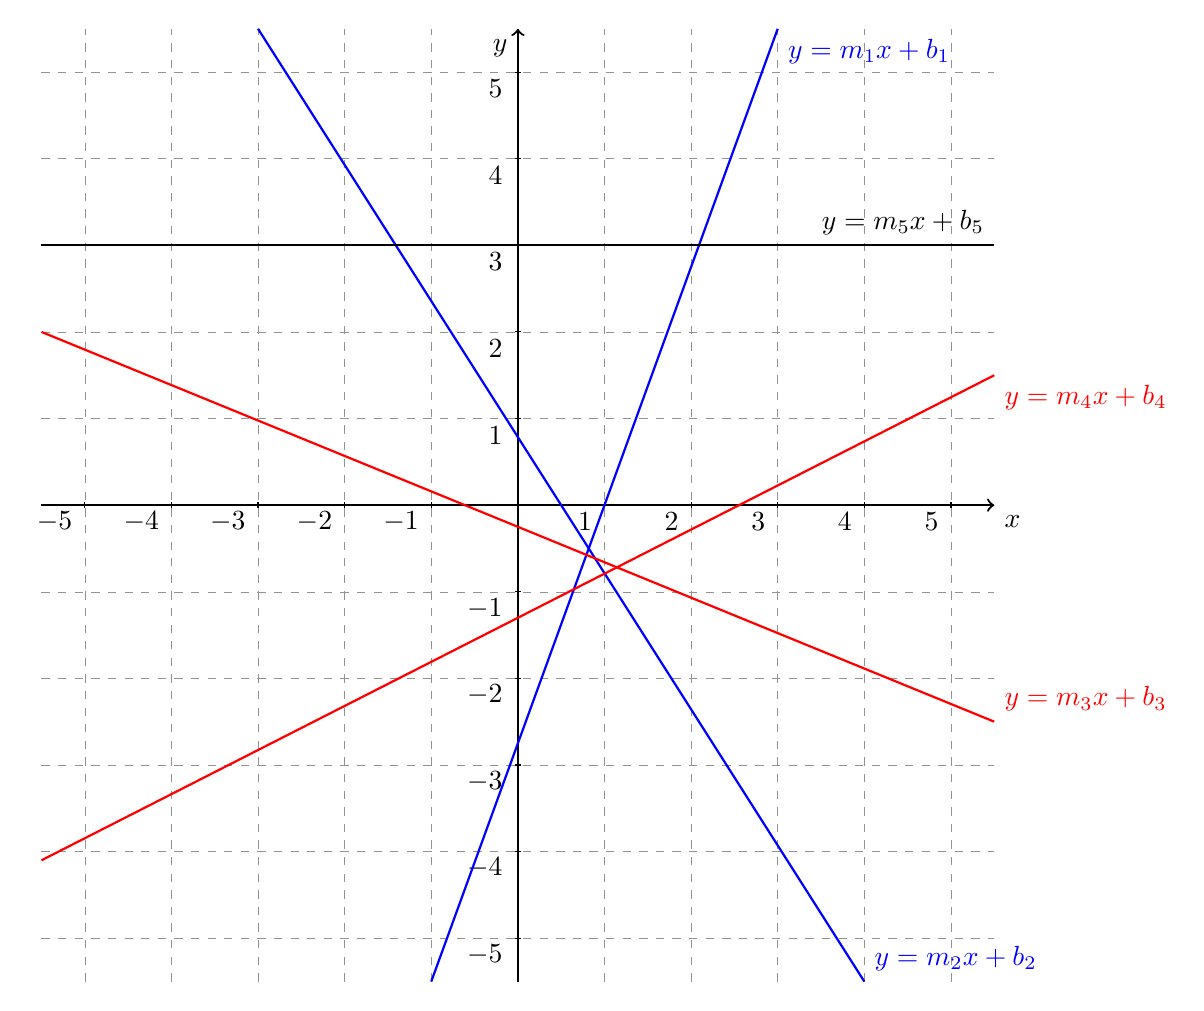
\begin{tikzpicture}[y=1.1cm, x=1.1cm,font=\sffamily]
    % bounds
    \def\lowX{-5.5}
    \pgfmathtruncatemacro\startX{round(0.5+\lowX)}
    \pgfmathsetmacro\nextXValue{int(\startX+1)}
    \def\highX{5.5}
    \def\lowY{-5.5}
    \def\highY{5.5}
    \pgfmathsetmacro\nextYValue{int(\lowY+1)}
    % ticks
    \draw[step = 1, gray, very thin,dashed,opacity=0.85] (\lowX, \lowY) grid ( \highX,\highY);
    % axis
    \draw[thick,->] (\lowX,0) -- coordinate (x axis mid) (\highX,0) node[anchor = north west] {$x$};
    \draw[thick,->] (0,\lowY) -- coordinate (y axis mid) (0,\highY) node[anchor = north east] {$y$};
    \foreach \y in {-5,-4,...,-1,1,2,...,\highY} {
      \draw (1pt, \y) -- (-1pt, \y) node[yshift=-6,xshift=-1,anchor=east] {$\y$};
    }
    \foreach \x in {-5,-4,...,-1,1,2,...,\highX} {
      \draw (\x,1pt) -- (\x,-1pt) node[yshift=-5,xshift=-1,anchor=east] {$\x$};
    }
        
    % Draw some lines and label them.
    \draw[thick, blue] (  -1,-5.5) -- (  3, 5.5) node[anchor=north west] {$y=m_1 x + b_1$};
    \draw[thick, blue] (  -3, 5.5) -- (  4,-5.5) node[anchor=south west] {$y=m_2 x + b_2$};
    \draw[thick,  red] (-5.5,   2) -- (5.5,-2.5) node[anchor=south west] {$y=m_3 x + b_3$};
    \draw[thick,  red] (-5.5,-4.1) -- (5.5, 1.5) node[anchor=north west] {$y=m_4 x + b_4$};
    \draw[thick,black] (-5.5, 3.0) -- (5.5, 3.0) node[anchor=south east] {$y=m_5 x + b_5$};
  \end{tikzpicture}

  \clearpage

\item For each question below the function, Larry($x$), is defined to be
  \begin{eqnarray*}
    \mathrm{Larry}(x) & = & \frac{1}{2} (x-1)^2+2.
  \end{eqnarray*}
  \begin{subproblem}
  \item Make a sketch of Larry.

    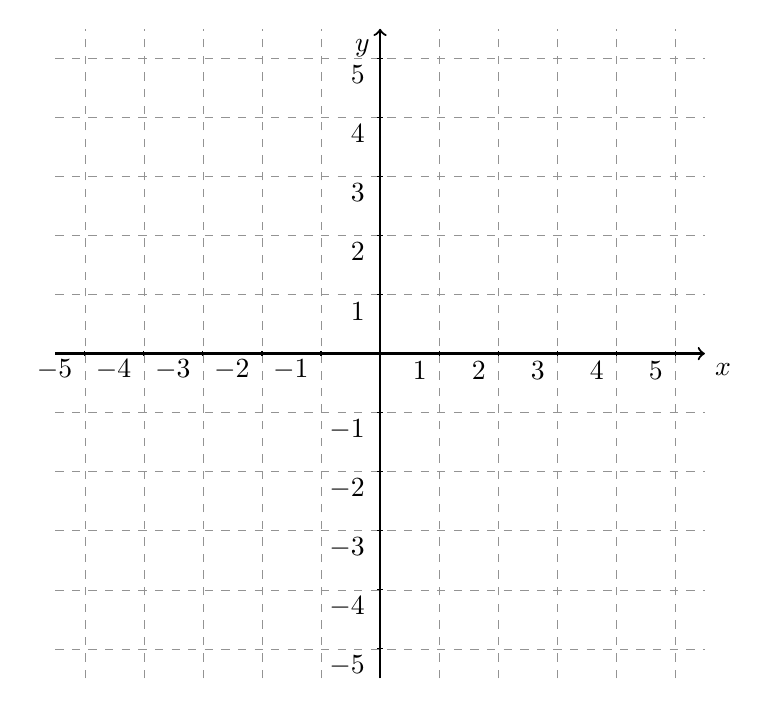
\begin{tikzpicture}[y=0.75cm, x=0.75cm,font=\sffamily]
      % bounds
      \def\lowX{-5.5}
      \pgfmathtruncatemacro\startX{round(0.5+\lowX)}
      \pgfmathsetmacro\nextXValue{int(\startX+1)}
      \def\highX{5.5}
      \def\lowY{-5.5}
      \def\highY{5.5}
      \pgfmathsetmacro\nextYValue{int(\lowY+1)}
      % ticks
      \draw[step = 1, gray, very thin,dashed,opacity=0.85] (\lowX, \lowY) grid ( \highX,\highY);
      % axis
      \draw[thick,->] (\lowX,0) -- coordinate (x axis mid) (\highX,0) node[anchor = north west] {$x$};
      \draw[thick,->] (0,\lowY) -- coordinate (y axis mid) (0,\highY) node[anchor = north east] {$y$};
      \foreach \y in {-5,-4,...,-1,1,2,...,\highY} {
        \draw (1pt, \y) -- (-1pt, \y) node[yshift=-6,xshift=-1,anchor=east] {$\y$};
      }
      \foreach \x in {-5,-4,...,-1,1,2,...,\highX} {
        \draw (\x,1pt) -- (\x,-1pt) node[yshift=-5,xshift=-1,anchor=east] {$\x$};
      }
        
    \end{tikzpicture}

  \item Determine the average rate of change of Larry from $x=-2$ to
    $x=3$. Add a sketch of the secant line for these points on your
    sketch above.

    \vfill

  \item Determine a value of $x_0$ where the average rate of change
    from $x=2$ to $x=x_0$ is zero. Add the a sketch of the resulting
    secant line for these points on your sketch above.

    \vfill

  \item Is there any value of $x=a$ where you cannot find another
    point so that the resulting average rate of change is zero?
    Explain your reasoning.

    \vspace{2em}


  \end{subproblem}

\end{problem}

\postClass

\begin{problem}
\item Briefly state two ideas from today's class.
  \begin{itemize}
  \item
  \item
  \end{itemize}
\item The growth rate for a population is the change in the number of
  individuals per unit time. The per-capita growth rate is the growth
  rate divided by the total number of individuals in the population.
  Suppose that the per-capita growth rate for a particular species is
  approximated as a linear function. It is estimated that when the
  population is near zero the per-capita growth rate is highest due to
  a lack of competition and approaches 0.5 (the time units are
  hours). When the population approaches 1,000 the per-capita growth
  rate is estimated to be zero the death rate and birth rate are
  balanced, and the total growth rate is zero.
  \begin{subproblem}
    \item What are the units for the per capita growth rate?
    \item Is the slope of the per-capita growth rate positive or
      negative? Explain why your answer makes sense given the physical
      situation.
    \item Determine the relationship that gives the per-capita growth
      rate as a function of the population, $p$.
    \item Make a sketch of the graph of the per-capita growth
      rate. (Make sure to annotate your graph and label your axes.)
    \item What happens to the per-capita growth rate as the population
      increases? Why might this happen?
    \item Determine the values where the per-capita growth rate is
      negative. Why would the per-capita growth rate be negative?
  \end{subproblem}
\end{problem}


%%% Local Variables:
%%% mode: latex
%%% TeX-master: "../labManual"
%%% End:


%=========================================================================
% Start of activity on linear models
%=========================================================================
\preClass{Linear Models}

\begin{problem}
\item A chemical reaction has a single reactant that breaks down, 
  and the resulting reaction produces two different
  products. It is estimated that for each gram of the reactant that
  $\frac{1}{3}$g of the first product is produced and $\frac{1}{6}$g
  of the original reactant remains. Everything else that remains is
  the second product.
  \begin{subproblem}
  \item Write down all of the relevant information that is given in the
    statement above.
    \vfill
  \item If you start with four grams of reactant how many grams of the
    reactant will you get in the end?
    \vfill
  \item If you start with four grams of reactant how much of each
    product do you get?  (Keep in mind that mass is
    conserved so you have to have the same total mass that you started
    with.)
    \vfill
  \item Determine the number of grams of the reactants will result
    when you start with $x$ grams of reactant.
    \vfill
  \item Determine the number of grams of the products will result when
    you start with $x$ grams of reactant.
    \vfill
  \end{subproblem}
\end{problem}


\actTitle{Modeling With Linear Functions}
\begin{problem}

\item The time required to bake ceramics depends on the mass of the
  ceramic. It is estimated to be a linear relationship between the
  time and mass. \textbf{The goal is to determine the time required to
    bake a ceramic sample given its mass.}
  \begin{subproblem}
    \item Should there be a positive or negative slope for the
      relationship? Briefly justify your answer.
      \vspace{2em}

    \item With respect to the costs, would you prefer a larger or
      smaller slope for the relationship? Briefly justify your answer.
      \vspace{2em}

    \item Samples are run, and it is estimated that the baking time
      for a ceramic whose mass is 2,000g is five hours. It is
      estimated that the baking time for a ceramic whose mass is
      3,000g is five and a half hours. Determine the baking time given
      the mass.
      \vfill
      \vfill

    \item A sample ceramic will be tested, and its mass is
      4,500g. How long would you expect it to take to bake the
      ceramic?
      \vfill

  \end{subproblem}

  \clearpage

\item Alice was born on the same day as her father, Bob. This year
  Bob's age is three times Alice's age. In fifteen years, Bob will be
  twice his daughter's age. What are their ages this year?
  \begin{subproblem}
  \item Let Alice's age this year be denoted as $A$, and let Bob's age
    this year be denoted as $B$. Write the algebraic expression that
    indicates that Bob's age is three times Alice's age.  
    \label{question:aliceBobCurrentAge}
    \vspace{2em}
  \item If Alice's age is now $A$ what will her age be in fifteen
    years?  
    \vspace{2em}
  \item If Bob's age is now $B$ what will his age be in fifteen years?
    \vspace{2em}
  \item Use the two previous expressions, and write out the algebraic
    expression that indicates that Bob's future age will be twice
    Alice's future age.
    \label{question:aliceBobFutureAge}
    \vspace{2em}
  \item Use the two expressions from parts
    \ref{question:aliceBobCurrentAge} and \ref{question:aliceBobFutureAge} 
    to draw a sketch of the two linear relationships. Assume that
    Bob's age is a function of Alice's age, and the horizontal axis
    will Alice's age. Will the system have a solution that makes
    sense? 
    \vfill

  \item Use the two expressions from parts
    \ref{question:aliceBobCurrentAge} and \ref{question:aliceBobFutureAge} 
    to determine Alice's and Bob's age.
    \vfill
  \end{subproblem}

\clearpage

\item Trucks are unloaded at a warehouse, and during the summer it is
  estimated that it takes longer to unload a truck if the weather is
  warmer. When the temperature is 22C it is estimated that it takes
  sixty minutes to unload a truck. For each increase of one degree
  Celsius it is estimated to take four additional minutes to unload a
  truck.
  \begin{subproblem}
    \item How long will it take to unload a truck if the temperature
      is 23C?
      \vspace{2em}
    \item How long will it take to unload a truck if the temperature
      is 24C?
      \vspace{2em}
    \item How long will it take to unload a truck given a temperature
      of T degrees Celsius?
      \vfill
  \end{subproblem}

  \clearpage

\item In the previous problem it was assumed that the truck was being
  unloaded during the summer. In the winter the relationship between
  unloading time and the temperature is different. When the
  temperature is 5C it is estimated that it takes fifty minutes to
  unload a truck, and for each decrease on one degree Celsius it is
  estimated to take three additional minutes to unload the truck.
  \begin{subproblem}
    \item Determine how long it will take to unload the truck for any
      temperature less than 5C.
      \vfill
    \item At what temperature should you switch from using the
      formula on the previous problem to using the formula above?
      \vfill
      \vfill
    \item Write out the formula to determine the time required to
      unload the truck given \textbf{any} temperature in Celsius.
      \vspace{3em}
    \item What is the shortest time to unload a time and what is the
      best temperature to unload a truck?  
      \vspace{2em}
  \end{subproblem}

\end{problem}

\postClass

\begin{problem}
\item Briefly state two ideas from today's class.
  \begin{itemize}
  \item 
  \item 
  \end{itemize}
\item 
  \begin{subproblem}
    \item
  \end{subproblem}
\end{problem}



%=========================================================================
% Start of 
%=========================================================================
\preClass{Graphs of Functions}

\begin{problem}
\item Two populations of different species of bacteria interact. The
  number of bacteria (in millions) in the first population is given by
  \begin{eqnarray*}
    B(t) & = & 10 + t^2,
  \end{eqnarray*}
  where $t$ is the time in days since the beginning of the year.  The
  number of bacteria (in millions) in the second population is given by
  \begin{eqnarray*}
    C(t) & = & 10+(t-2)^2,
  \end{eqnarray*}
  where $t$ is the time in days since the beginning of the year.
  \begin{subproblem}
  \item Make a sketch of the two functions below.
    \vfill
  \item A researcher decides to alter the situation and adds 5 million
    bacteria to the first population given by $B(t)$. Determine a
    formula for the altered population. Make a sketch of the original
    and altered populations below.
    \vfill
  \end{subproblem}

\end{problem}


\actTitle{Graphs of Functions}
\begin{problem}
\item The height of a certain tree changes by the relationship
  \begin{eqnarray*}
    h(t) & = & \sqrt{\frac{t}{3}},
  \end{eqnarray*}
  where $t$ is the time in years from when the seed was germinated. 
  \begin{subproblem}
  \item Make a sketch of the height of a tree as a function of time.
    \vfill
  \item Two seeds are planted, and the second seed germinates one year
    after the first is germinated. Determine the formulas for the
    height of the two trees with respect to the time that the first
    seed is germinated. Make a sketch of the two functions on the same
    graph.
    \vfill
  \item A new strain of the tree is developed that grows twice as fast
    as the original. Determine the formula that will give the height
    of the new strain. Make a sketch comparing the height of the
    original and the new strains.
    \vfill
  \end{subproblem}

  \clearpage

\item A function is defined to be
  \begin{eqnarray*}
    f(x) & = & |x|.
  \end{eqnarray*}
  \begin{subproblem}
  \item Make a sketch of the function on the axes below.
  \item Make a sketch of the following new functions on the graph as
    well with clear annotations:
    \begin{eqnarray*}
      g(x) & = & f(3x), \\
      h(x) & = & f(x)+2, \\
      p(x) & = & f(x+2), \\
      q(x) & = & 3f(x).
    \end{eqnarray*}

    \scalebox{0.95}{%% Creator: Matplotlib, PGF backend
%%
%% To include the figure in your LaTeX document, write
%%   \input{<filename>.pgf}
%%
%% Make sure the required packages are loaded in your preamble
%%   \usepackage{pgf}
%%
%% Figures using additional raster images can only be included by \input if
%% they are in the same directory as the main LaTeX file. For loading figures
%% from other directories you can use the `import` package
%%   \usepackage{import}
%% and then include the figures with
%%   \import{<path to file>}{<filename>.pgf}
%%
%% Matplotlib used the following preamble
%%   \usepackage{fontspec}
%%   \setmainfont{Bitstream Vera Serif}
%%   \setsansfont{Bitstream Vera Sans}
%%   \setmonofont{Bitstream Vera Sans Mono}
%%
\begingroup%
\makeatletter%
\begin{pgfpicture}%
\pgfpathrectangle{\pgfpointorigin}{\pgfqpoint{8.000000in}{6.000000in}}%
\pgfusepath{use as bounding box, clip}%
\begin{pgfscope}%
\pgfsetbuttcap%
\pgfsetmiterjoin%
\definecolor{currentfill}{rgb}{1.000000,1.000000,1.000000}%
\pgfsetfillcolor{currentfill}%
\pgfsetlinewidth{0.000000pt}%
\definecolor{currentstroke}{rgb}{1.000000,1.000000,1.000000}%
\pgfsetstrokecolor{currentstroke}%
\pgfsetdash{}{0pt}%
\pgfpathmoveto{\pgfqpoint{0.000000in}{0.000000in}}%
\pgfpathlineto{\pgfqpoint{8.000000in}{0.000000in}}%
\pgfpathlineto{\pgfqpoint{8.000000in}{6.000000in}}%
\pgfpathlineto{\pgfqpoint{0.000000in}{6.000000in}}%
\pgfpathclose%
\pgfusepath{fill}%
\end{pgfscope}%
\begin{pgfscope}%
\pgfsetbuttcap%
\pgfsetmiterjoin%
\definecolor{currentfill}{rgb}{1.000000,1.000000,1.000000}%
\pgfsetfillcolor{currentfill}%
\pgfsetlinewidth{0.000000pt}%
\definecolor{currentstroke}{rgb}{0.000000,0.000000,0.000000}%
\pgfsetstrokecolor{currentstroke}%
\pgfsetstrokeopacity{0.000000}%
\pgfsetdash{}{0pt}%
\pgfpathmoveto{\pgfqpoint{1.000000in}{0.600000in}}%
\pgfpathlineto{\pgfqpoint{7.200000in}{0.600000in}}%
\pgfpathlineto{\pgfqpoint{7.200000in}{5.400000in}}%
\pgfpathlineto{\pgfqpoint{1.000000in}{5.400000in}}%
\pgfpathclose%
\pgfusepath{fill}%
\end{pgfscope}%
\begin{pgfscope}%
\pgfsetrectcap%
\pgfsetmiterjoin%
\pgfsetlinewidth{0.000000pt}%
\definecolor{currentstroke}{rgb}{0.000000,0.000000,0.000000}%
\pgfsetstrokecolor{currentstroke}%
\pgfsetstrokeopacity{0.000000}%
\pgfsetdash{}{0pt}%
\pgfpathmoveto{\pgfqpoint{1.000000in}{5.400000in}}%
\pgfpathlineto{\pgfqpoint{7.200000in}{5.400000in}}%
\pgfusepath{}%
\end{pgfscope}%
\begin{pgfscope}%
\pgfsetrectcap%
\pgfsetmiterjoin%
\pgfsetlinewidth{0.000000pt}%
\definecolor{currentstroke}{rgb}{0.000000,0.000000,0.000000}%
\pgfsetstrokecolor{currentstroke}%
\pgfsetstrokeopacity{0.000000}%
\pgfsetdash{}{0pt}%
\pgfpathmoveto{\pgfqpoint{7.200000in}{0.600000in}}%
\pgfpathlineto{\pgfqpoint{7.200000in}{5.400000in}}%
\pgfusepath{}%
\end{pgfscope}%
\begin{pgfscope}%
\pgfsetrectcap%
\pgfsetmiterjoin%
\pgfsetlinewidth{1.003750pt}%
\definecolor{currentstroke}{rgb}{0.000000,0.000000,0.000000}%
\pgfsetstrokecolor{currentstroke}%
\pgfsetdash{}{0pt}%
\pgfpathmoveto{\pgfqpoint{1.000000in}{3.000000in}}%
\pgfpathlineto{\pgfqpoint{7.200000in}{3.000000in}}%
\pgfusepath{stroke}%
\end{pgfscope}%
\begin{pgfscope}%
\pgfsetrectcap%
\pgfsetmiterjoin%
\pgfsetlinewidth{1.003750pt}%
\definecolor{currentstroke}{rgb}{0.000000,0.000000,0.000000}%
\pgfsetstrokecolor{currentstroke}%
\pgfsetdash{}{0pt}%
\pgfpathmoveto{\pgfqpoint{4.100000in}{0.600000in}}%
\pgfpathlineto{\pgfqpoint{4.100000in}{5.400000in}}%
\pgfusepath{stroke}%
\end{pgfscope}%
\begin{pgfscope}%
\pgfsetbuttcap%
\pgfsetroundjoin%
\pgfsetlinewidth{0.501875pt}%
\definecolor{currentstroke}{rgb}{0.000000,0.000000,0.000000}%
\pgfsetstrokecolor{currentstroke}%
\pgfsetdash{{1.000000pt}{3.000000pt}}{0.000000pt}%
\pgfpathmoveto{\pgfqpoint{1.060784in}{0.600000in}}%
\pgfpathlineto{\pgfqpoint{1.060784in}{5.400000in}}%
\pgfusepath{stroke}%
\end{pgfscope}%
\begin{pgfscope}%
\pgfsetbuttcap%
\pgfsetroundjoin%
\definecolor{currentfill}{rgb}{0.000000,0.000000,0.000000}%
\pgfsetfillcolor{currentfill}%
\pgfsetlinewidth{0.501875pt}%
\definecolor{currentstroke}{rgb}{0.000000,0.000000,0.000000}%
\pgfsetstrokecolor{currentstroke}%
\pgfsetdash{}{0pt}%
\pgfsys@defobject{currentmarker}{\pgfqpoint{0.000000in}{0.000000in}}{\pgfqpoint{0.000000in}{0.055556in}}{%
\pgfpathmoveto{\pgfqpoint{0.000000in}{0.000000in}}%
\pgfpathlineto{\pgfqpoint{0.000000in}{0.055556in}}%
\pgfusepath{stroke,fill}%
}%
\begin{pgfscope}%
\pgfsys@transformshift{1.060784in}{3.000000in}%
\pgfsys@useobject{currentmarker}{}%
\end{pgfscope}%
\end{pgfscope}%
\begin{pgfscope}%
\pgftext[x=1.060784in,y=2.944444in,,top]{\sffamily\fontsize{12.000000}{14.400000}\selectfont -5}%
\end{pgfscope}%
\begin{pgfscope}%
\pgfsetbuttcap%
\pgfsetroundjoin%
\pgfsetlinewidth{0.501875pt}%
\definecolor{currentstroke}{rgb}{0.000000,0.000000,0.000000}%
\pgfsetstrokecolor{currentstroke}%
\pgfsetdash{{1.000000pt}{3.000000pt}}{0.000000pt}%
\pgfpathmoveto{\pgfqpoint{1.668627in}{0.600000in}}%
\pgfpathlineto{\pgfqpoint{1.668627in}{5.400000in}}%
\pgfusepath{stroke}%
\end{pgfscope}%
\begin{pgfscope}%
\pgfsetbuttcap%
\pgfsetroundjoin%
\definecolor{currentfill}{rgb}{0.000000,0.000000,0.000000}%
\pgfsetfillcolor{currentfill}%
\pgfsetlinewidth{0.501875pt}%
\definecolor{currentstroke}{rgb}{0.000000,0.000000,0.000000}%
\pgfsetstrokecolor{currentstroke}%
\pgfsetdash{}{0pt}%
\pgfsys@defobject{currentmarker}{\pgfqpoint{0.000000in}{0.000000in}}{\pgfqpoint{0.000000in}{0.055556in}}{%
\pgfpathmoveto{\pgfqpoint{0.000000in}{0.000000in}}%
\pgfpathlineto{\pgfqpoint{0.000000in}{0.055556in}}%
\pgfusepath{stroke,fill}%
}%
\begin{pgfscope}%
\pgfsys@transformshift{1.668627in}{3.000000in}%
\pgfsys@useobject{currentmarker}{}%
\end{pgfscope}%
\end{pgfscope}%
\begin{pgfscope}%
\pgftext[x=1.668627in,y=2.944444in,,top]{\sffamily\fontsize{12.000000}{14.400000}\selectfont -4}%
\end{pgfscope}%
\begin{pgfscope}%
\pgfsetbuttcap%
\pgfsetroundjoin%
\pgfsetlinewidth{0.501875pt}%
\definecolor{currentstroke}{rgb}{0.000000,0.000000,0.000000}%
\pgfsetstrokecolor{currentstroke}%
\pgfsetdash{{1.000000pt}{3.000000pt}}{0.000000pt}%
\pgfpathmoveto{\pgfqpoint{2.276471in}{0.600000in}}%
\pgfpathlineto{\pgfqpoint{2.276471in}{5.400000in}}%
\pgfusepath{stroke}%
\end{pgfscope}%
\begin{pgfscope}%
\pgfsetbuttcap%
\pgfsetroundjoin%
\definecolor{currentfill}{rgb}{0.000000,0.000000,0.000000}%
\pgfsetfillcolor{currentfill}%
\pgfsetlinewidth{0.501875pt}%
\definecolor{currentstroke}{rgb}{0.000000,0.000000,0.000000}%
\pgfsetstrokecolor{currentstroke}%
\pgfsetdash{}{0pt}%
\pgfsys@defobject{currentmarker}{\pgfqpoint{0.000000in}{0.000000in}}{\pgfqpoint{0.000000in}{0.055556in}}{%
\pgfpathmoveto{\pgfqpoint{0.000000in}{0.000000in}}%
\pgfpathlineto{\pgfqpoint{0.000000in}{0.055556in}}%
\pgfusepath{stroke,fill}%
}%
\begin{pgfscope}%
\pgfsys@transformshift{2.276471in}{3.000000in}%
\pgfsys@useobject{currentmarker}{}%
\end{pgfscope}%
\end{pgfscope}%
\begin{pgfscope}%
\pgftext[x=2.276471in,y=2.944444in,,top]{\sffamily\fontsize{12.000000}{14.400000}\selectfont -3}%
\end{pgfscope}%
\begin{pgfscope}%
\pgfsetbuttcap%
\pgfsetroundjoin%
\pgfsetlinewidth{0.501875pt}%
\definecolor{currentstroke}{rgb}{0.000000,0.000000,0.000000}%
\pgfsetstrokecolor{currentstroke}%
\pgfsetdash{{1.000000pt}{3.000000pt}}{0.000000pt}%
\pgfpathmoveto{\pgfqpoint{2.884314in}{0.600000in}}%
\pgfpathlineto{\pgfqpoint{2.884314in}{5.400000in}}%
\pgfusepath{stroke}%
\end{pgfscope}%
\begin{pgfscope}%
\pgfsetbuttcap%
\pgfsetroundjoin%
\definecolor{currentfill}{rgb}{0.000000,0.000000,0.000000}%
\pgfsetfillcolor{currentfill}%
\pgfsetlinewidth{0.501875pt}%
\definecolor{currentstroke}{rgb}{0.000000,0.000000,0.000000}%
\pgfsetstrokecolor{currentstroke}%
\pgfsetdash{}{0pt}%
\pgfsys@defobject{currentmarker}{\pgfqpoint{0.000000in}{0.000000in}}{\pgfqpoint{0.000000in}{0.055556in}}{%
\pgfpathmoveto{\pgfqpoint{0.000000in}{0.000000in}}%
\pgfpathlineto{\pgfqpoint{0.000000in}{0.055556in}}%
\pgfusepath{stroke,fill}%
}%
\begin{pgfscope}%
\pgfsys@transformshift{2.884314in}{3.000000in}%
\pgfsys@useobject{currentmarker}{}%
\end{pgfscope}%
\end{pgfscope}%
\begin{pgfscope}%
\pgftext[x=2.884314in,y=2.944444in,,top]{\sffamily\fontsize{12.000000}{14.400000}\selectfont -2}%
\end{pgfscope}%
\begin{pgfscope}%
\pgfsetbuttcap%
\pgfsetroundjoin%
\pgfsetlinewidth{0.501875pt}%
\definecolor{currentstroke}{rgb}{0.000000,0.000000,0.000000}%
\pgfsetstrokecolor{currentstroke}%
\pgfsetdash{{1.000000pt}{3.000000pt}}{0.000000pt}%
\pgfpathmoveto{\pgfqpoint{3.492157in}{0.600000in}}%
\pgfpathlineto{\pgfqpoint{3.492157in}{5.400000in}}%
\pgfusepath{stroke}%
\end{pgfscope}%
\begin{pgfscope}%
\pgfsetbuttcap%
\pgfsetroundjoin%
\definecolor{currentfill}{rgb}{0.000000,0.000000,0.000000}%
\pgfsetfillcolor{currentfill}%
\pgfsetlinewidth{0.501875pt}%
\definecolor{currentstroke}{rgb}{0.000000,0.000000,0.000000}%
\pgfsetstrokecolor{currentstroke}%
\pgfsetdash{}{0pt}%
\pgfsys@defobject{currentmarker}{\pgfqpoint{0.000000in}{0.000000in}}{\pgfqpoint{0.000000in}{0.055556in}}{%
\pgfpathmoveto{\pgfqpoint{0.000000in}{0.000000in}}%
\pgfpathlineto{\pgfqpoint{0.000000in}{0.055556in}}%
\pgfusepath{stroke,fill}%
}%
\begin{pgfscope}%
\pgfsys@transformshift{3.492157in}{3.000000in}%
\pgfsys@useobject{currentmarker}{}%
\end{pgfscope}%
\end{pgfscope}%
\begin{pgfscope}%
\pgftext[x=3.492157in,y=2.944444in,,top]{\sffamily\fontsize{12.000000}{14.400000}\selectfont -1}%
\end{pgfscope}%
\begin{pgfscope}%
\pgfsetbuttcap%
\pgfsetroundjoin%
\pgfsetlinewidth{0.501875pt}%
\definecolor{currentstroke}{rgb}{0.000000,0.000000,0.000000}%
\pgfsetstrokecolor{currentstroke}%
\pgfsetdash{{1.000000pt}{3.000000pt}}{0.000000pt}%
\pgfpathmoveto{\pgfqpoint{4.100000in}{0.600000in}}%
\pgfpathlineto{\pgfqpoint{4.100000in}{5.400000in}}%
\pgfusepath{stroke}%
\end{pgfscope}%
\begin{pgfscope}%
\pgfsetbuttcap%
\pgfsetroundjoin%
\definecolor{currentfill}{rgb}{0.000000,0.000000,0.000000}%
\pgfsetfillcolor{currentfill}%
\pgfsetlinewidth{0.501875pt}%
\definecolor{currentstroke}{rgb}{0.000000,0.000000,0.000000}%
\pgfsetstrokecolor{currentstroke}%
\pgfsetdash{}{0pt}%
\pgfsys@defobject{currentmarker}{\pgfqpoint{0.000000in}{0.000000in}}{\pgfqpoint{0.000000in}{0.055556in}}{%
\pgfpathmoveto{\pgfqpoint{0.000000in}{0.000000in}}%
\pgfpathlineto{\pgfqpoint{0.000000in}{0.055556in}}%
\pgfusepath{stroke,fill}%
}%
\begin{pgfscope}%
\pgfsys@transformshift{4.100000in}{3.000000in}%
\pgfsys@useobject{currentmarker}{}%
\end{pgfscope}%
\end{pgfscope}%
\begin{pgfscope}%
\pgftext[x=4.100000in,y=2.944444in,,top]{\sffamily\fontsize{12.000000}{14.400000}\selectfont 0}%
\end{pgfscope}%
\begin{pgfscope}%
\pgfsetbuttcap%
\pgfsetroundjoin%
\pgfsetlinewidth{0.501875pt}%
\definecolor{currentstroke}{rgb}{0.000000,0.000000,0.000000}%
\pgfsetstrokecolor{currentstroke}%
\pgfsetdash{{1.000000pt}{3.000000pt}}{0.000000pt}%
\pgfpathmoveto{\pgfqpoint{4.707843in}{0.600000in}}%
\pgfpathlineto{\pgfqpoint{4.707843in}{5.400000in}}%
\pgfusepath{stroke}%
\end{pgfscope}%
\begin{pgfscope}%
\pgfsetbuttcap%
\pgfsetroundjoin%
\definecolor{currentfill}{rgb}{0.000000,0.000000,0.000000}%
\pgfsetfillcolor{currentfill}%
\pgfsetlinewidth{0.501875pt}%
\definecolor{currentstroke}{rgb}{0.000000,0.000000,0.000000}%
\pgfsetstrokecolor{currentstroke}%
\pgfsetdash{}{0pt}%
\pgfsys@defobject{currentmarker}{\pgfqpoint{0.000000in}{0.000000in}}{\pgfqpoint{0.000000in}{0.055556in}}{%
\pgfpathmoveto{\pgfqpoint{0.000000in}{0.000000in}}%
\pgfpathlineto{\pgfqpoint{0.000000in}{0.055556in}}%
\pgfusepath{stroke,fill}%
}%
\begin{pgfscope}%
\pgfsys@transformshift{4.707843in}{3.000000in}%
\pgfsys@useobject{currentmarker}{}%
\end{pgfscope}%
\end{pgfscope}%
\begin{pgfscope}%
\pgftext[x=4.707843in,y=2.944444in,,top]{\sffamily\fontsize{12.000000}{14.400000}\selectfont 1}%
\end{pgfscope}%
\begin{pgfscope}%
\pgfsetbuttcap%
\pgfsetroundjoin%
\pgfsetlinewidth{0.501875pt}%
\definecolor{currentstroke}{rgb}{0.000000,0.000000,0.000000}%
\pgfsetstrokecolor{currentstroke}%
\pgfsetdash{{1.000000pt}{3.000000pt}}{0.000000pt}%
\pgfpathmoveto{\pgfqpoint{5.315686in}{0.600000in}}%
\pgfpathlineto{\pgfqpoint{5.315686in}{5.400000in}}%
\pgfusepath{stroke}%
\end{pgfscope}%
\begin{pgfscope}%
\pgfsetbuttcap%
\pgfsetroundjoin%
\definecolor{currentfill}{rgb}{0.000000,0.000000,0.000000}%
\pgfsetfillcolor{currentfill}%
\pgfsetlinewidth{0.501875pt}%
\definecolor{currentstroke}{rgb}{0.000000,0.000000,0.000000}%
\pgfsetstrokecolor{currentstroke}%
\pgfsetdash{}{0pt}%
\pgfsys@defobject{currentmarker}{\pgfqpoint{0.000000in}{0.000000in}}{\pgfqpoint{0.000000in}{0.055556in}}{%
\pgfpathmoveto{\pgfqpoint{0.000000in}{0.000000in}}%
\pgfpathlineto{\pgfqpoint{0.000000in}{0.055556in}}%
\pgfusepath{stroke,fill}%
}%
\begin{pgfscope}%
\pgfsys@transformshift{5.315686in}{3.000000in}%
\pgfsys@useobject{currentmarker}{}%
\end{pgfscope}%
\end{pgfscope}%
\begin{pgfscope}%
\pgftext[x=5.315686in,y=2.944444in,,top]{\sffamily\fontsize{12.000000}{14.400000}\selectfont 2}%
\end{pgfscope}%
\begin{pgfscope}%
\pgfsetbuttcap%
\pgfsetroundjoin%
\pgfsetlinewidth{0.501875pt}%
\definecolor{currentstroke}{rgb}{0.000000,0.000000,0.000000}%
\pgfsetstrokecolor{currentstroke}%
\pgfsetdash{{1.000000pt}{3.000000pt}}{0.000000pt}%
\pgfpathmoveto{\pgfqpoint{5.923529in}{0.600000in}}%
\pgfpathlineto{\pgfqpoint{5.923529in}{5.400000in}}%
\pgfusepath{stroke}%
\end{pgfscope}%
\begin{pgfscope}%
\pgfsetbuttcap%
\pgfsetroundjoin%
\definecolor{currentfill}{rgb}{0.000000,0.000000,0.000000}%
\pgfsetfillcolor{currentfill}%
\pgfsetlinewidth{0.501875pt}%
\definecolor{currentstroke}{rgb}{0.000000,0.000000,0.000000}%
\pgfsetstrokecolor{currentstroke}%
\pgfsetdash{}{0pt}%
\pgfsys@defobject{currentmarker}{\pgfqpoint{0.000000in}{0.000000in}}{\pgfqpoint{0.000000in}{0.055556in}}{%
\pgfpathmoveto{\pgfqpoint{0.000000in}{0.000000in}}%
\pgfpathlineto{\pgfqpoint{0.000000in}{0.055556in}}%
\pgfusepath{stroke,fill}%
}%
\begin{pgfscope}%
\pgfsys@transformshift{5.923529in}{3.000000in}%
\pgfsys@useobject{currentmarker}{}%
\end{pgfscope}%
\end{pgfscope}%
\begin{pgfscope}%
\pgftext[x=5.923529in,y=2.944444in,,top]{\sffamily\fontsize{12.000000}{14.400000}\selectfont 3}%
\end{pgfscope}%
\begin{pgfscope}%
\pgfsetbuttcap%
\pgfsetroundjoin%
\pgfsetlinewidth{0.501875pt}%
\definecolor{currentstroke}{rgb}{0.000000,0.000000,0.000000}%
\pgfsetstrokecolor{currentstroke}%
\pgfsetdash{{1.000000pt}{3.000000pt}}{0.000000pt}%
\pgfpathmoveto{\pgfqpoint{6.531373in}{0.600000in}}%
\pgfpathlineto{\pgfqpoint{6.531373in}{5.400000in}}%
\pgfusepath{stroke}%
\end{pgfscope}%
\begin{pgfscope}%
\pgfsetbuttcap%
\pgfsetroundjoin%
\definecolor{currentfill}{rgb}{0.000000,0.000000,0.000000}%
\pgfsetfillcolor{currentfill}%
\pgfsetlinewidth{0.501875pt}%
\definecolor{currentstroke}{rgb}{0.000000,0.000000,0.000000}%
\pgfsetstrokecolor{currentstroke}%
\pgfsetdash{}{0pt}%
\pgfsys@defobject{currentmarker}{\pgfqpoint{0.000000in}{0.000000in}}{\pgfqpoint{0.000000in}{0.055556in}}{%
\pgfpathmoveto{\pgfqpoint{0.000000in}{0.000000in}}%
\pgfpathlineto{\pgfqpoint{0.000000in}{0.055556in}}%
\pgfusepath{stroke,fill}%
}%
\begin{pgfscope}%
\pgfsys@transformshift{6.531373in}{3.000000in}%
\pgfsys@useobject{currentmarker}{}%
\end{pgfscope}%
\end{pgfscope}%
\begin{pgfscope}%
\pgftext[x=6.531373in,y=2.944444in,,top]{\sffamily\fontsize{12.000000}{14.400000}\selectfont 4}%
\end{pgfscope}%
\begin{pgfscope}%
\pgfsetbuttcap%
\pgfsetroundjoin%
\pgfsetlinewidth{0.501875pt}%
\definecolor{currentstroke}{rgb}{0.000000,0.000000,0.000000}%
\pgfsetstrokecolor{currentstroke}%
\pgfsetdash{{1.000000pt}{3.000000pt}}{0.000000pt}%
\pgfpathmoveto{\pgfqpoint{7.139216in}{0.600000in}}%
\pgfpathlineto{\pgfqpoint{7.139216in}{5.400000in}}%
\pgfusepath{stroke}%
\end{pgfscope}%
\begin{pgfscope}%
\pgfsetbuttcap%
\pgfsetroundjoin%
\definecolor{currentfill}{rgb}{0.000000,0.000000,0.000000}%
\pgfsetfillcolor{currentfill}%
\pgfsetlinewidth{0.501875pt}%
\definecolor{currentstroke}{rgb}{0.000000,0.000000,0.000000}%
\pgfsetstrokecolor{currentstroke}%
\pgfsetdash{}{0pt}%
\pgfsys@defobject{currentmarker}{\pgfqpoint{0.000000in}{0.000000in}}{\pgfqpoint{0.000000in}{0.055556in}}{%
\pgfpathmoveto{\pgfqpoint{0.000000in}{0.000000in}}%
\pgfpathlineto{\pgfqpoint{0.000000in}{0.055556in}}%
\pgfusepath{stroke,fill}%
}%
\begin{pgfscope}%
\pgfsys@transformshift{7.139216in}{3.000000in}%
\pgfsys@useobject{currentmarker}{}%
\end{pgfscope}%
\end{pgfscope}%
\begin{pgfscope}%
\pgftext[x=7.139216in,y=2.944444in,,top]{\sffamily\fontsize{12.000000}{14.400000}\selectfont 5}%
\end{pgfscope}%
\begin{pgfscope}%
\pgftext[x=6.890000in,y=2.760000in,,top]{\sffamily\fontsize{12.000000}{14.400000}\selectfont x}%
\end{pgfscope}%
\begin{pgfscope}%
\pgfsetbuttcap%
\pgfsetroundjoin%
\pgfsetlinewidth{0.501875pt}%
\definecolor{currentstroke}{rgb}{0.000000,0.000000,0.000000}%
\pgfsetstrokecolor{currentstroke}%
\pgfsetdash{{1.000000pt}{3.000000pt}}{0.000000pt}%
\pgfpathmoveto{\pgfqpoint{1.000000in}{0.647059in}}%
\pgfpathlineto{\pgfqpoint{7.200000in}{0.647059in}}%
\pgfusepath{stroke}%
\end{pgfscope}%
\begin{pgfscope}%
\pgfsetbuttcap%
\pgfsetroundjoin%
\definecolor{currentfill}{rgb}{0.000000,0.000000,0.000000}%
\pgfsetfillcolor{currentfill}%
\pgfsetlinewidth{0.501875pt}%
\definecolor{currentstroke}{rgb}{0.000000,0.000000,0.000000}%
\pgfsetstrokecolor{currentstroke}%
\pgfsetdash{}{0pt}%
\pgfsys@defobject{currentmarker}{\pgfqpoint{0.000000in}{0.000000in}}{\pgfqpoint{0.055556in}{0.000000in}}{%
\pgfpathmoveto{\pgfqpoint{0.000000in}{0.000000in}}%
\pgfpathlineto{\pgfqpoint{0.055556in}{0.000000in}}%
\pgfusepath{stroke,fill}%
}%
\begin{pgfscope}%
\pgfsys@transformshift{4.100000in}{0.647059in}%
\pgfsys@useobject{currentmarker}{}%
\end{pgfscope}%
\end{pgfscope}%
\begin{pgfscope}%
\pgftext[x=4.044444in,y=0.647059in,right,]{\sffamily\fontsize{12.000000}{14.400000}\selectfont -5}%
\end{pgfscope}%
\begin{pgfscope}%
\pgfsetbuttcap%
\pgfsetroundjoin%
\pgfsetlinewidth{0.501875pt}%
\definecolor{currentstroke}{rgb}{0.000000,0.000000,0.000000}%
\pgfsetstrokecolor{currentstroke}%
\pgfsetdash{{1.000000pt}{3.000000pt}}{0.000000pt}%
\pgfpathmoveto{\pgfqpoint{1.000000in}{1.117647in}}%
\pgfpathlineto{\pgfqpoint{7.200000in}{1.117647in}}%
\pgfusepath{stroke}%
\end{pgfscope}%
\begin{pgfscope}%
\pgfsetbuttcap%
\pgfsetroundjoin%
\definecolor{currentfill}{rgb}{0.000000,0.000000,0.000000}%
\pgfsetfillcolor{currentfill}%
\pgfsetlinewidth{0.501875pt}%
\definecolor{currentstroke}{rgb}{0.000000,0.000000,0.000000}%
\pgfsetstrokecolor{currentstroke}%
\pgfsetdash{}{0pt}%
\pgfsys@defobject{currentmarker}{\pgfqpoint{0.000000in}{0.000000in}}{\pgfqpoint{0.055556in}{0.000000in}}{%
\pgfpathmoveto{\pgfqpoint{0.000000in}{0.000000in}}%
\pgfpathlineto{\pgfqpoint{0.055556in}{0.000000in}}%
\pgfusepath{stroke,fill}%
}%
\begin{pgfscope}%
\pgfsys@transformshift{4.100000in}{1.117647in}%
\pgfsys@useobject{currentmarker}{}%
\end{pgfscope}%
\end{pgfscope}%
\begin{pgfscope}%
\pgftext[x=4.044444in,y=1.117647in,right,]{\sffamily\fontsize{12.000000}{14.400000}\selectfont -4}%
\end{pgfscope}%
\begin{pgfscope}%
\pgfsetbuttcap%
\pgfsetroundjoin%
\pgfsetlinewidth{0.501875pt}%
\definecolor{currentstroke}{rgb}{0.000000,0.000000,0.000000}%
\pgfsetstrokecolor{currentstroke}%
\pgfsetdash{{1.000000pt}{3.000000pt}}{0.000000pt}%
\pgfpathmoveto{\pgfqpoint{1.000000in}{1.588235in}}%
\pgfpathlineto{\pgfqpoint{7.200000in}{1.588235in}}%
\pgfusepath{stroke}%
\end{pgfscope}%
\begin{pgfscope}%
\pgfsetbuttcap%
\pgfsetroundjoin%
\definecolor{currentfill}{rgb}{0.000000,0.000000,0.000000}%
\pgfsetfillcolor{currentfill}%
\pgfsetlinewidth{0.501875pt}%
\definecolor{currentstroke}{rgb}{0.000000,0.000000,0.000000}%
\pgfsetstrokecolor{currentstroke}%
\pgfsetdash{}{0pt}%
\pgfsys@defobject{currentmarker}{\pgfqpoint{0.000000in}{0.000000in}}{\pgfqpoint{0.055556in}{0.000000in}}{%
\pgfpathmoveto{\pgfqpoint{0.000000in}{0.000000in}}%
\pgfpathlineto{\pgfqpoint{0.055556in}{0.000000in}}%
\pgfusepath{stroke,fill}%
}%
\begin{pgfscope}%
\pgfsys@transformshift{4.100000in}{1.588235in}%
\pgfsys@useobject{currentmarker}{}%
\end{pgfscope}%
\end{pgfscope}%
\begin{pgfscope}%
\pgftext[x=4.044444in,y=1.588235in,right,]{\sffamily\fontsize{12.000000}{14.400000}\selectfont -3}%
\end{pgfscope}%
\begin{pgfscope}%
\pgfsetbuttcap%
\pgfsetroundjoin%
\pgfsetlinewidth{0.501875pt}%
\definecolor{currentstroke}{rgb}{0.000000,0.000000,0.000000}%
\pgfsetstrokecolor{currentstroke}%
\pgfsetdash{{1.000000pt}{3.000000pt}}{0.000000pt}%
\pgfpathmoveto{\pgfqpoint{1.000000in}{2.058824in}}%
\pgfpathlineto{\pgfqpoint{7.200000in}{2.058824in}}%
\pgfusepath{stroke}%
\end{pgfscope}%
\begin{pgfscope}%
\pgfsetbuttcap%
\pgfsetroundjoin%
\definecolor{currentfill}{rgb}{0.000000,0.000000,0.000000}%
\pgfsetfillcolor{currentfill}%
\pgfsetlinewidth{0.501875pt}%
\definecolor{currentstroke}{rgb}{0.000000,0.000000,0.000000}%
\pgfsetstrokecolor{currentstroke}%
\pgfsetdash{}{0pt}%
\pgfsys@defobject{currentmarker}{\pgfqpoint{0.000000in}{0.000000in}}{\pgfqpoint{0.055556in}{0.000000in}}{%
\pgfpathmoveto{\pgfqpoint{0.000000in}{0.000000in}}%
\pgfpathlineto{\pgfqpoint{0.055556in}{0.000000in}}%
\pgfusepath{stroke,fill}%
}%
\begin{pgfscope}%
\pgfsys@transformshift{4.100000in}{2.058824in}%
\pgfsys@useobject{currentmarker}{}%
\end{pgfscope}%
\end{pgfscope}%
\begin{pgfscope}%
\pgftext[x=4.044444in,y=2.058824in,right,]{\sffamily\fontsize{12.000000}{14.400000}\selectfont -2}%
\end{pgfscope}%
\begin{pgfscope}%
\pgfsetbuttcap%
\pgfsetroundjoin%
\pgfsetlinewidth{0.501875pt}%
\definecolor{currentstroke}{rgb}{0.000000,0.000000,0.000000}%
\pgfsetstrokecolor{currentstroke}%
\pgfsetdash{{1.000000pt}{3.000000pt}}{0.000000pt}%
\pgfpathmoveto{\pgfqpoint{1.000000in}{2.529412in}}%
\pgfpathlineto{\pgfqpoint{7.200000in}{2.529412in}}%
\pgfusepath{stroke}%
\end{pgfscope}%
\begin{pgfscope}%
\pgfsetbuttcap%
\pgfsetroundjoin%
\definecolor{currentfill}{rgb}{0.000000,0.000000,0.000000}%
\pgfsetfillcolor{currentfill}%
\pgfsetlinewidth{0.501875pt}%
\definecolor{currentstroke}{rgb}{0.000000,0.000000,0.000000}%
\pgfsetstrokecolor{currentstroke}%
\pgfsetdash{}{0pt}%
\pgfsys@defobject{currentmarker}{\pgfqpoint{0.000000in}{0.000000in}}{\pgfqpoint{0.055556in}{0.000000in}}{%
\pgfpathmoveto{\pgfqpoint{0.000000in}{0.000000in}}%
\pgfpathlineto{\pgfqpoint{0.055556in}{0.000000in}}%
\pgfusepath{stroke,fill}%
}%
\begin{pgfscope}%
\pgfsys@transformshift{4.100000in}{2.529412in}%
\pgfsys@useobject{currentmarker}{}%
\end{pgfscope}%
\end{pgfscope}%
\begin{pgfscope}%
\pgftext[x=4.044444in,y=2.529412in,right,]{\sffamily\fontsize{12.000000}{14.400000}\selectfont -1}%
\end{pgfscope}%
\begin{pgfscope}%
\pgfsetbuttcap%
\pgfsetroundjoin%
\pgfsetlinewidth{0.501875pt}%
\definecolor{currentstroke}{rgb}{0.000000,0.000000,0.000000}%
\pgfsetstrokecolor{currentstroke}%
\pgfsetdash{{1.000000pt}{3.000000pt}}{0.000000pt}%
\pgfpathmoveto{\pgfqpoint{1.000000in}{3.000000in}}%
\pgfpathlineto{\pgfqpoint{7.200000in}{3.000000in}}%
\pgfusepath{stroke}%
\end{pgfscope}%
\begin{pgfscope}%
\pgfsetbuttcap%
\pgfsetroundjoin%
\definecolor{currentfill}{rgb}{0.000000,0.000000,0.000000}%
\pgfsetfillcolor{currentfill}%
\pgfsetlinewidth{0.501875pt}%
\definecolor{currentstroke}{rgb}{0.000000,0.000000,0.000000}%
\pgfsetstrokecolor{currentstroke}%
\pgfsetdash{}{0pt}%
\pgfsys@defobject{currentmarker}{\pgfqpoint{0.000000in}{0.000000in}}{\pgfqpoint{0.055556in}{0.000000in}}{%
\pgfpathmoveto{\pgfqpoint{0.000000in}{0.000000in}}%
\pgfpathlineto{\pgfqpoint{0.055556in}{0.000000in}}%
\pgfusepath{stroke,fill}%
}%
\begin{pgfscope}%
\pgfsys@transformshift{4.100000in}{3.000000in}%
\pgfsys@useobject{currentmarker}{}%
\end{pgfscope}%
\end{pgfscope}%
\begin{pgfscope}%
\pgftext[x=4.044444in,y=3.000000in,right,]{\sffamily\fontsize{12.000000}{14.400000}\selectfont 0}%
\end{pgfscope}%
\begin{pgfscope}%
\pgfsetbuttcap%
\pgfsetroundjoin%
\pgfsetlinewidth{0.501875pt}%
\definecolor{currentstroke}{rgb}{0.000000,0.000000,0.000000}%
\pgfsetstrokecolor{currentstroke}%
\pgfsetdash{{1.000000pt}{3.000000pt}}{0.000000pt}%
\pgfpathmoveto{\pgfqpoint{1.000000in}{3.470588in}}%
\pgfpathlineto{\pgfqpoint{7.200000in}{3.470588in}}%
\pgfusepath{stroke}%
\end{pgfscope}%
\begin{pgfscope}%
\pgfsetbuttcap%
\pgfsetroundjoin%
\definecolor{currentfill}{rgb}{0.000000,0.000000,0.000000}%
\pgfsetfillcolor{currentfill}%
\pgfsetlinewidth{0.501875pt}%
\definecolor{currentstroke}{rgb}{0.000000,0.000000,0.000000}%
\pgfsetstrokecolor{currentstroke}%
\pgfsetdash{}{0pt}%
\pgfsys@defobject{currentmarker}{\pgfqpoint{0.000000in}{0.000000in}}{\pgfqpoint{0.055556in}{0.000000in}}{%
\pgfpathmoveto{\pgfqpoint{0.000000in}{0.000000in}}%
\pgfpathlineto{\pgfqpoint{0.055556in}{0.000000in}}%
\pgfusepath{stroke,fill}%
}%
\begin{pgfscope}%
\pgfsys@transformshift{4.100000in}{3.470588in}%
\pgfsys@useobject{currentmarker}{}%
\end{pgfscope}%
\end{pgfscope}%
\begin{pgfscope}%
\pgftext[x=4.044444in,y=3.470588in,right,]{\sffamily\fontsize{12.000000}{14.400000}\selectfont 1}%
\end{pgfscope}%
\begin{pgfscope}%
\pgfsetbuttcap%
\pgfsetroundjoin%
\pgfsetlinewidth{0.501875pt}%
\definecolor{currentstroke}{rgb}{0.000000,0.000000,0.000000}%
\pgfsetstrokecolor{currentstroke}%
\pgfsetdash{{1.000000pt}{3.000000pt}}{0.000000pt}%
\pgfpathmoveto{\pgfqpoint{1.000000in}{3.941176in}}%
\pgfpathlineto{\pgfqpoint{7.200000in}{3.941176in}}%
\pgfusepath{stroke}%
\end{pgfscope}%
\begin{pgfscope}%
\pgfsetbuttcap%
\pgfsetroundjoin%
\definecolor{currentfill}{rgb}{0.000000,0.000000,0.000000}%
\pgfsetfillcolor{currentfill}%
\pgfsetlinewidth{0.501875pt}%
\definecolor{currentstroke}{rgb}{0.000000,0.000000,0.000000}%
\pgfsetstrokecolor{currentstroke}%
\pgfsetdash{}{0pt}%
\pgfsys@defobject{currentmarker}{\pgfqpoint{0.000000in}{0.000000in}}{\pgfqpoint{0.055556in}{0.000000in}}{%
\pgfpathmoveto{\pgfqpoint{0.000000in}{0.000000in}}%
\pgfpathlineto{\pgfqpoint{0.055556in}{0.000000in}}%
\pgfusepath{stroke,fill}%
}%
\begin{pgfscope}%
\pgfsys@transformshift{4.100000in}{3.941176in}%
\pgfsys@useobject{currentmarker}{}%
\end{pgfscope}%
\end{pgfscope}%
\begin{pgfscope}%
\pgftext[x=4.044444in,y=3.941176in,right,]{\sffamily\fontsize{12.000000}{14.400000}\selectfont 2}%
\end{pgfscope}%
\begin{pgfscope}%
\pgfsetbuttcap%
\pgfsetroundjoin%
\pgfsetlinewidth{0.501875pt}%
\definecolor{currentstroke}{rgb}{0.000000,0.000000,0.000000}%
\pgfsetstrokecolor{currentstroke}%
\pgfsetdash{{1.000000pt}{3.000000pt}}{0.000000pt}%
\pgfpathmoveto{\pgfqpoint{1.000000in}{4.411765in}}%
\pgfpathlineto{\pgfqpoint{7.200000in}{4.411765in}}%
\pgfusepath{stroke}%
\end{pgfscope}%
\begin{pgfscope}%
\pgfsetbuttcap%
\pgfsetroundjoin%
\definecolor{currentfill}{rgb}{0.000000,0.000000,0.000000}%
\pgfsetfillcolor{currentfill}%
\pgfsetlinewidth{0.501875pt}%
\definecolor{currentstroke}{rgb}{0.000000,0.000000,0.000000}%
\pgfsetstrokecolor{currentstroke}%
\pgfsetdash{}{0pt}%
\pgfsys@defobject{currentmarker}{\pgfqpoint{0.000000in}{0.000000in}}{\pgfqpoint{0.055556in}{0.000000in}}{%
\pgfpathmoveto{\pgfqpoint{0.000000in}{0.000000in}}%
\pgfpathlineto{\pgfqpoint{0.055556in}{0.000000in}}%
\pgfusepath{stroke,fill}%
}%
\begin{pgfscope}%
\pgfsys@transformshift{4.100000in}{4.411765in}%
\pgfsys@useobject{currentmarker}{}%
\end{pgfscope}%
\end{pgfscope}%
\begin{pgfscope}%
\pgftext[x=4.044444in,y=4.411765in,right,]{\sffamily\fontsize{12.000000}{14.400000}\selectfont 3}%
\end{pgfscope}%
\begin{pgfscope}%
\pgfsetbuttcap%
\pgfsetroundjoin%
\pgfsetlinewidth{0.501875pt}%
\definecolor{currentstroke}{rgb}{0.000000,0.000000,0.000000}%
\pgfsetstrokecolor{currentstroke}%
\pgfsetdash{{1.000000pt}{3.000000pt}}{0.000000pt}%
\pgfpathmoveto{\pgfqpoint{1.000000in}{4.882353in}}%
\pgfpathlineto{\pgfqpoint{7.200000in}{4.882353in}}%
\pgfusepath{stroke}%
\end{pgfscope}%
\begin{pgfscope}%
\pgfsetbuttcap%
\pgfsetroundjoin%
\definecolor{currentfill}{rgb}{0.000000,0.000000,0.000000}%
\pgfsetfillcolor{currentfill}%
\pgfsetlinewidth{0.501875pt}%
\definecolor{currentstroke}{rgb}{0.000000,0.000000,0.000000}%
\pgfsetstrokecolor{currentstroke}%
\pgfsetdash{}{0pt}%
\pgfsys@defobject{currentmarker}{\pgfqpoint{0.000000in}{0.000000in}}{\pgfqpoint{0.055556in}{0.000000in}}{%
\pgfpathmoveto{\pgfqpoint{0.000000in}{0.000000in}}%
\pgfpathlineto{\pgfqpoint{0.055556in}{0.000000in}}%
\pgfusepath{stroke,fill}%
}%
\begin{pgfscope}%
\pgfsys@transformshift{4.100000in}{4.882353in}%
\pgfsys@useobject{currentmarker}{}%
\end{pgfscope}%
\end{pgfscope}%
\begin{pgfscope}%
\pgftext[x=4.044444in,y=4.882353in,right,]{\sffamily\fontsize{12.000000}{14.400000}\selectfont 4}%
\end{pgfscope}%
\begin{pgfscope}%
\pgfsetbuttcap%
\pgfsetroundjoin%
\pgfsetlinewidth{0.501875pt}%
\definecolor{currentstroke}{rgb}{0.000000,0.000000,0.000000}%
\pgfsetstrokecolor{currentstroke}%
\pgfsetdash{{1.000000pt}{3.000000pt}}{0.000000pt}%
\pgfpathmoveto{\pgfqpoint{1.000000in}{5.352941in}}%
\pgfpathlineto{\pgfqpoint{7.200000in}{5.352941in}}%
\pgfusepath{stroke}%
\end{pgfscope}%
\begin{pgfscope}%
\pgfsetbuttcap%
\pgfsetroundjoin%
\definecolor{currentfill}{rgb}{0.000000,0.000000,0.000000}%
\pgfsetfillcolor{currentfill}%
\pgfsetlinewidth{0.501875pt}%
\definecolor{currentstroke}{rgb}{0.000000,0.000000,0.000000}%
\pgfsetstrokecolor{currentstroke}%
\pgfsetdash{}{0pt}%
\pgfsys@defobject{currentmarker}{\pgfqpoint{0.000000in}{0.000000in}}{\pgfqpoint{0.055556in}{0.000000in}}{%
\pgfpathmoveto{\pgfqpoint{0.000000in}{0.000000in}}%
\pgfpathlineto{\pgfqpoint{0.055556in}{0.000000in}}%
\pgfusepath{stroke,fill}%
}%
\begin{pgfscope}%
\pgfsys@transformshift{4.100000in}{5.352941in}%
\pgfsys@useobject{currentmarker}{}%
\end{pgfscope}%
\end{pgfscope}%
\begin{pgfscope}%
\pgftext[x=4.044444in,y=5.352941in,right,]{\sffamily\fontsize{12.000000}{14.400000}\selectfont 5}%
\end{pgfscope}%
\begin{pgfscope}%
\pgftext[x=3.790000in,y=5.160000in,,bottom,rotate=90.000000]{\sffamily\fontsize{12.000000}{14.400000}\selectfont y}%
\end{pgfscope}%
\begin{pgfscope}%
\pgftext[x=4.100000in,y=5.469444in,,base]{\sffamily\fontsize{14.400000}{17.280000}\selectfont Comparing Shifted Functions}%
\end{pgfscope}%
\end{pgfpicture}%
\makeatother%
\endgroup%
}

  \end{subproblem}
\end{problem}

\postClass

\begin{problem}
\item Briefly state two ideas from today's class.
  \begin{itemize}
  \item 
  \item 
  \end{itemize}
\item 
  \begin{subproblem}
    \item
  \end{subproblem}
\end{problem}


%%% Local Variables:
%%% mode: latex
%%% TeX-master: "../labManual"
%%% End:



%=========================================================================
% Start of activity on piece wise defined functions and max/min
%=========================================================================
\preClass{Introduction to Piece-wise Defined Functions}

\begin{problem}
\item The graph of a function, $g$, is shown shown below:

  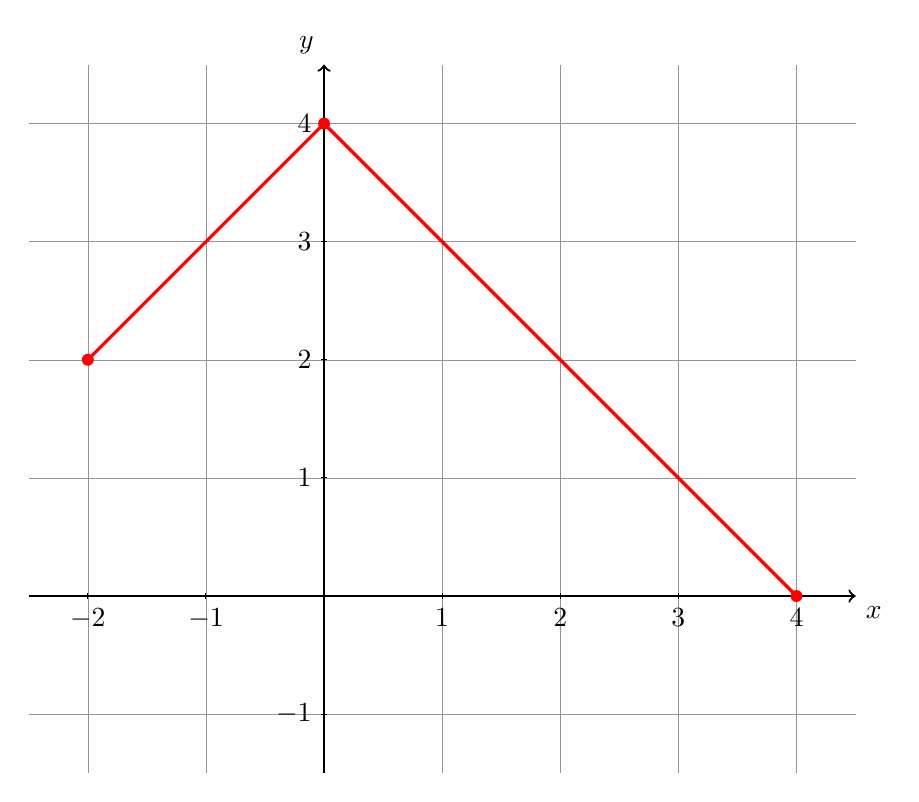
\begin{tikzpicture}[y=1.5cm, x=1.5cm,font=\sffamily]
    % ticks
    \draw[step = 1, gray, very thin,opacity=0.85] (-2.5, -1.5) grid ( 4.5, 4.5);
 	% axis
	\draw[thick,->] (-2.5,0) -- coordinate (x axis mid) (4.5,0) 
          node[anchor = north west] {$x$};
    \draw[thick,->] (0,-1.5) -- coordinate (y axis mid) (0,4.5) 
          node[anchor = south east] {$y$};
    \foreach \y in {-1,1,2,3,4} {
      \draw (1pt, \y) -- (-1pt, \y) node[anchor = east] {$\y$};
    }
    \foreach \x in {-2,-1,1,2,3,4} {
      \draw (\x,1pt) -- (\x,-1pt) node[anchor = north] {$\x$};
    }
    % Draw the function
    \draw [red, very thick] plot coordinates {(-2,2) (0,4) (4,0)};
    \fill[red] (-2, 2) circle [radius=0.5ex];
    \fill[red] ( 0, 4) circle [radius=0.5ex];
    \fill[red] ( 4,0) circle [radius=0.5ex];
  \end{tikzpicture}

  \begin{subproblem}
  \item Determine the domain and range of the function.
    \vfill
  \item Determine the formula for the function if $x\geq -2$ and
    $x<0$.
    \vfill
  \item Determine the formula for the function if $x> 0$ and
    $x\leq 4$.
    \vfill
  \item For what values of $x$ is the function increasing?
    \vspace{2em}
  \item For what values of $x$ is the function decreasing?
    \vspace{2em}
  \end{subproblem}

\end{problem}


\actTitle{Piece-wise Defined Functions}
\begin{problem}
\item A piece of metal is initially at 20C. It is placed in a hot
  furnace for twenty-five minutes, and its temperature is raised to
  200C. It is then removed from the oven and placed in cold water and
  cooled to room temperature.. After five minutes it is placed back
  into the furnace, and the process is repeated twice for a total
  number of three cycles. Make a sketch of the graph of the
  temperature of the piece of metal on the axes below.

    \hspace{-7em}
    \begin{tikzpicture}[y=0.03cm, x=0.14cm,font=\sffamily]
        % bounds
        \def\lowX{-0.5}
        \pgfmathtruncatemacro\startX{round(0.5+\lowX)}
        \pgfmathsetmacro\nextXValue{int(\startX+1)}
        \def\highX{100.5}
        \def\lowY{-0.5}
        \def\highY{220.0}
        \pgfmathsetmacro\nextYValue{int(\lowY+1)}
        % ticks
        \draw[xstep = 10,ystep=50, gray, very thin,dashed,opacity=0.85] (\lowX, \lowY) grid ( \highX,\highY);
      % axis
      \draw[thick,->] (\lowX,0) -- coordinate (x axis mid) (\highX,0) node[anchor = north west] {Time (Min)};
        \draw[thick,->] (0,\lowY) -- coordinate (y axis mid) (0,\highY) node[anchor = north east] {Temp. (C)};
        \foreach \y in {50,100,...,\highY} {
          \draw (1pt, \y) -- (-1pt, \y) node[yshift=-6,xshift=-1,anchor=east] {$\y$};
        }
        \foreach \x in {10,20,...,\highX} {
          \draw (\x,1pt) -- (\x,-1pt) node[yshift=-5,xshift=-1,anchor=east] {$\x$};
        }
        %\draw (0,5.5) node [anchor=south] {Comparing Shifted Functions};
      \end{tikzpicture}

      \begin{subproblem}
      \item What is the range and domain of the function?
        \vfill
      \item Determine the values of the time where the function is
        increasing.
        \vfill
      \item Determine the values of the time where the function is
        decreasing.  
        \vfill
      \end{subproblem}

      \clearpage
\item The questions below refer to the function whose graph is given
  below.

  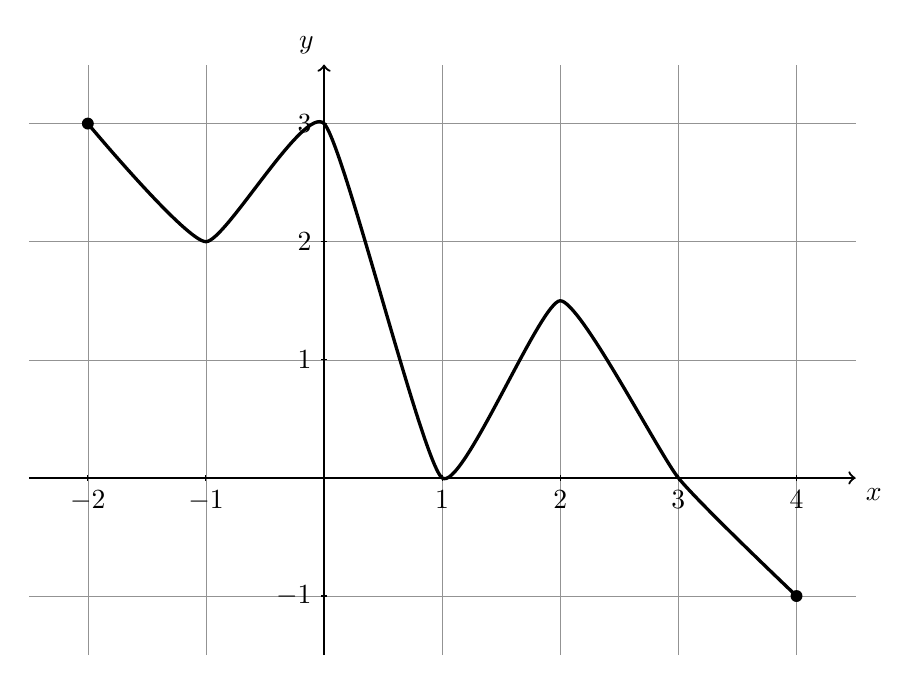
\begin{tikzpicture}[y=1.5cm, x=1.5cm,font=\sffamily]
    % ticks
    \draw[step = 1, gray, very thin,opacity=0.85] (-2.5, -1.5) grid ( 4.5, 3.5);
 	% axis
	\draw[thick,->] (-2.5,0) -- coordinate (x axis mid) (4.5,0) 
          node[anchor = north west] {$x$};
    \draw[thick,->] (0,-1.5) -- coordinate (y axis mid) (0,3.5) 
          node[anchor = south east] {$y$};
    \foreach \y in {-1,1,2,3} {
      \draw (1pt, \y) -- (-1pt, \y) node[anchor = east] {$\y$};
    }
    \foreach \x in {-2,-1,1,2,3,4} {
      \draw (\x,1pt) -- (\x,-1pt) node[anchor = north] {$\x$};
    }
    % Draw the function
    \draw [black, very thick] plot [smooth, tension=0.3] coordinates {
      (-2,3) (-1,2) (0,3) (1,0) (2,1.5) (3,0) (4,-1)};
    \fill (-2, 3) circle [radius=0.5ex];
    \fill ( 4,-1) circle [radius=0.5ex];
  \end{tikzpicture}

  \begin{subproblem}
    \item Determine the domain and range of the function.
      \vfill
    \item Determine the values of $x$ where the function is
      increasing.
      \vfill
    \item Determine the values of $x$ where the function is
      decreasing.
      \vfill
  \end{subproblem}

  \clearpage

\item Make sketch of the graph of the function
  \begin{eqnarray*}
    \mathrm{Harold}(x) & = & \left\{
                             \begin{array}{l@{\hspace{3em}}rcccl}
                               \frac{1}{2}(x+2) & -2 & \leq & x & < &  0, \\
                               4-x^2            &  0 &   <  & x & < &  2, \\
                               -2(x-2)          &  2 & \leq & x & < & 4.
                             \end{array}
                             \right.
  \end{eqnarray*}
  Determine the domain and range of the function. Determine where the
  function is increasing. Also determine where it is decreasing.

    \begin{tikzpicture}[y=1.1cm, x=1.1cm,font=\sffamily]
        % bounds
        \def\lowX{-5.5}
        \pgfmathtruncatemacro\startX{round(0.5+\lowX)}
        \pgfmathsetmacro\nextXValue{int(\startX+1)}
        \def\highX{5.5}
        \def\lowY{-5.5}
        \def\highY{5.5}
        \pgfmathsetmacro\nextYValue{int(\lowY+1)}
        % ticks
        \draw[step = 1, gray, very thin,dashed,opacity=0.85] (\lowX, \lowY) grid ( \highX,\highY);
      % axis
      \draw[thick,->] (\lowX,0) -- coordinate (x axis mid) (\highX,0) node[anchor = north west] {$x$};
        \draw[thick,->] (0,\lowY) -- coordinate (y axis mid) (0,\highY) node[anchor = north east] {$y$};
        \foreach \y in {-5,-4,...,-1,1,2,...,\highY} {
          \draw (1pt, \y) -- (-1pt, \y) node[yshift=-6,xshift=-1,anchor=east] {$\y$};
        }
        \foreach \x in {-5,-4,...,-1,1,2,...,\highX} {
          \draw (\x,1pt) -- (\x,-1pt) node[yshift=-5,xshift=-1,anchor=east] {$\x$};
        }
        %\draw (0,5.5) node [anchor=south] {Comparing Shifted Functions};
      \end{tikzpicture}


\clearpage

\item Part of the graph of a function is given below. The function is
  even. Sketch the rest of the function. Determine the domain and
  range of the function.

    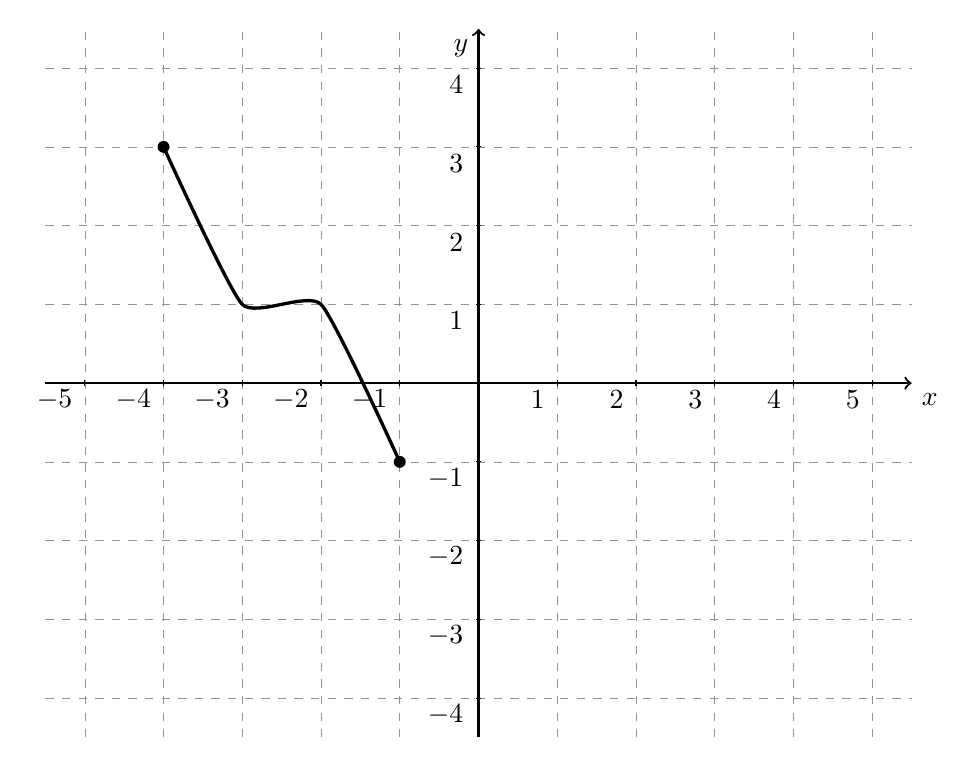
\begin{tikzpicture}[y=1.0cm, x=1.0cm,font=\sffamily]
        % bounds
        \def\lowX{-5.5}
        \pgfmathtruncatemacro\startX{round(0.5+\lowX)}
        \pgfmathsetmacro\nextXValue{int(\startX+1)}
        \def\highX{5.5}
        \def\lowY{-4.5}
        \def\highY{4.5}
        \pgfmathsetmacro\nextYValue{int(\lowY+1)}
        % ticks
        \draw[step = 1, gray, very thin,dashed,opacity=0.85] (\lowX, \lowY) grid ( \highX,\highY);
      % axis
      \draw[thick,->] (\lowX,0) -- coordinate (x axis mid) (\highX,0) node[anchor = north west] {$x$};
        \draw[thick,->] (0,\lowY) -- coordinate (y axis mid) (0,\highY) node[anchor = north east] {$y$};
        \foreach \y in {-4,-3,...,-1,1,2,...,\highY} {
          \draw (1pt, \y) -- (-1pt, \y) node[yshift=-6,xshift=-1,anchor=east] {$\y$};
        }
        \foreach \x in {-5,-4,...,-1,1,2,...,\highX} {
          \draw (\x,1pt) -- (\x,-1pt) node[yshift=-5,xshift=-1,anchor=east] {$\x$};
        }
        \draw [black, very thick] plot [smooth, tension=0.3] coordinates {
          (-4,3) (-3,1) (-2,1) (-1,-1)};
        \fill (-4, 3) circle [radius=0.5ex];
        \fill (-1,-1) circle [radius=0.5ex];

      \end{tikzpicture}

    \item Part of the graph of a function is given below. The function
      is odd. Sketch the rest of the function. Determine the domain
      and range of the function.

    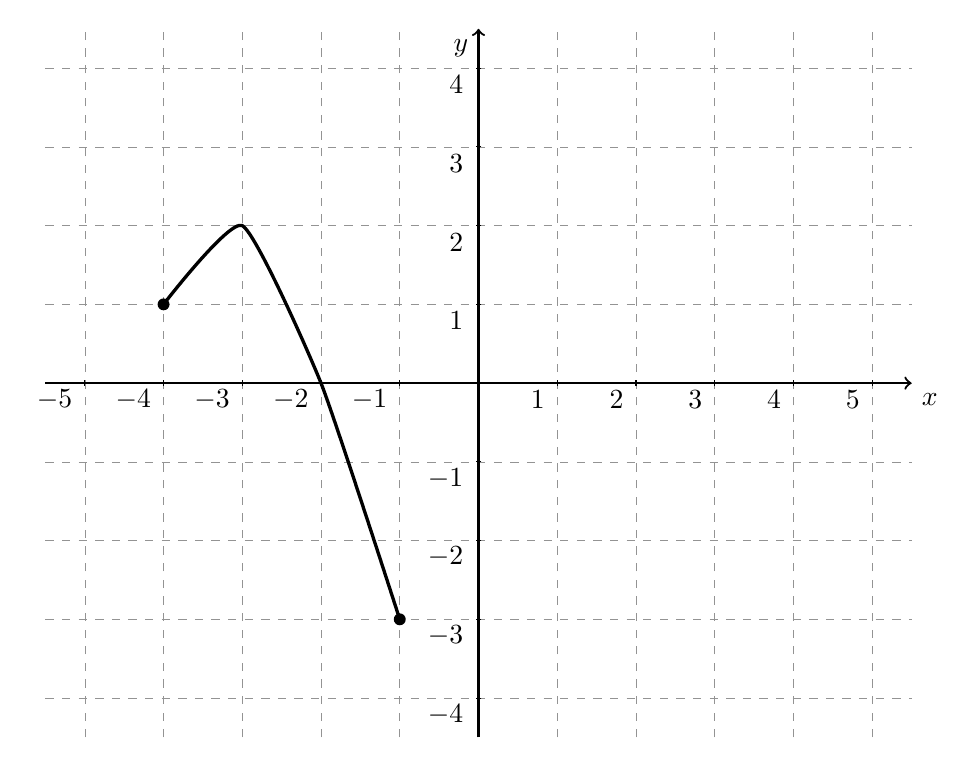
\begin{tikzpicture}[y=1.0cm, x=1.0cm,font=\sffamily]
        % bounds
        \def\lowX{-5.5}
        \pgfmathtruncatemacro\startX{round(0.5+\lowX)}
        \pgfmathsetmacro\nextXValue{int(\startX+1)}
        \def\highX{5.5}
        \def\lowY{-4.5}
        \def\highY{4.5}
        \pgfmathsetmacro\nextYValue{int(\lowY+1)}
        % ticks
        \draw[step = 1, gray, very thin,dashed,opacity=0.85] (\lowX, \lowY) grid ( \highX,\highY);
      % axis
      \draw[thick,->] (\lowX,0) -- coordinate (x axis mid) (\highX,0) node[anchor = north west] {$x$};
        \draw[thick,->] (0,\lowY) -- coordinate (y axis mid) (0,\highY) node[anchor = north east] {$y$};
        \foreach \y in {-4,-3,...,-1,1,2,...,\highY} {
          \draw (1pt, \y) -- (-1pt, \y) node[yshift=-6,xshift=-1,anchor=east] {$\y$};
        }
        \foreach \x in {-5,-4,...,-1,1,2,...,\highX} {
          \draw (\x,1pt) -- (\x,-1pt) node[yshift=-5,xshift=-1,anchor=east] {$\x$};
        }
        \draw [black, very thick] plot [smooth, tension=0.3] coordinates {
          (-4,1) (-3,2) (-2,-0) (-1,-3)};
        \fill (-4, 1) circle [radius=0.5ex];
        \fill (-1,-3) circle [radius=0.5ex];

      \end{tikzpicture}

      \clearpage

    \item A small company builds a set of solar panels. The amount of
      electricity produced is proportional to the intensity of sun
      light. When the sunlight is bright, 100,000 lux, the system
      produces 4,000 watts. On one day of operation there is a good
      deal of cloud cover, and the amount of sunlight varies linearly
      from 6am to noon from 0 lux to 50,000 lux. After noon it varies
      linearly to 0 lux at 6pm. On the second day the cycle repeats,
      but the maximum amount of light is 100,000 lux. Determine the
      amount of power produced by the panel at any time during the two
      days. (Include night time!)

      \vfill

\end{problem}

\postClass

\begin{problem}
\item Briefly state two ideas from today's class.
  \begin{itemize}
  \item 
  \item 
  \end{itemize}
\item 
  \begin{subproblem}
    \item
  \end{subproblem}
\end{problem}


%%% Local Variables:
%%% mode: latex
%%% TeX-master: "../labManual"
%%% End:



%=========================================================================
% Start of 
%=========================================================================
\preClass{Title}

\begin{problem}
\item
\end{problem}


\actTitle{title}
\begin{problem}
\item 
  \begin{subproblem}
    \item
  \end{subproblem}
\end{problem}

\postClass

\begin{problem}
\item Briefly state two ideas from today's class.
  \begin{itemize}
  \item 
  \item 
  \end{itemize}
\item 
  \begin{subproblem}
    \item
  \end{subproblem}
\end{problem}


%%% Local Variables:
%%% mode: latex
%%% TeX-master: "../labManual"
%%% End:



%=========================================================================
% Start of 
%=========================================================================
\preClass{Title}

\begin{problem}
\item
\end{problem}


\actTitle{title}
\begin{problem}
\item 
  \begin{subproblem}
    \item
  \end{subproblem}
\end{problem}

\postClass

\begin{problem}
\item Briefly state two ideas from today's class.
  \begin{itemize}
  \item 
  \item 
  \end{itemize}
\item 
  \begin{subproblem}
    \item
  \end{subproblem}
\end{problem}


%%% Local Variables:
%%% mode: latex
%%% TeX-master: "../labManual"
%%% End:



%=========================================================================
% Start of 
%=========================================================================
\preClass{Title}

\begin{problem}
\item
\end{problem}


\actTitle{title}
\begin{problem}
\item 
  \begin{subproblem}
    \item
  \end{subproblem}
\end{problem}

\postClass

\begin{problem}
\item Briefly state two ideas from today's class.
  \begin{itemize}
  \item 
  \item 
  \end{itemize}
\item 
  \begin{subproblem}
    \item
  \end{subproblem}
\end{problem}


%%% Local Variables:
%%% mode: latex
%%% TeX-master: "../labManual"
%%% End:



%%% Local Variables:
%%% mode: latex
%%% TeX-master: "../labManual"
%%% End:
